\documentclass[12pt, a4paper, oneside]{article}
\usepackage{amsmath, amsthm, amssymb, bm, graphicx, hyperref, mathrsfs}
\usepackage{geometry}
\usepackage{amsmath}
\newtheorem{theorem}{Theorem}
\newtheorem{lemma}{Lemma}
\usepackage{hyperref}
\usepackage{mathrsfs}
\usepackage[ruled, lined, linesnumbered, commentsnumbered, longend]{algorithm2e}
\usepackage{booktabs}
\usepackage{breqn}
\usepackage{natbib}
\usepackage{amsmath}
\numberwithin{equation}{section}
\usepackage[ruled,linesnumbered]{algorithm2e}
\usepackage[UTF8]{ctex}
\usepackage{subfigure}

\title{\textbf{Hierarchical heterogeneous analysis of high-dimensional data
		based on interactions}}
\author{Yan Ren \\ 2021103739}
\date{\today}
\linespread{1.5}
\newcounter{problemname}
\newenvironment{problem}{\stepcounter{problemname}\par\noindent\textsc{Problem \arabic{problemname}. }}{\\\par}
\newenvironment{solution}{\par\noindent\textsc{Solution. }}{\\\par}
\newenvironment{note}{\par\noindent\textsc{Note of Problem \arabic{problemname}. }}{\\\par}
\newcommand{\nysm}{Nystr$\ddot{\rm o}$m Method}
\geometry{a4paper, scale = 0.8}

\begin{document}
	
\maketitle
\newpage
\tableofcontents
\newpage

\section{Problem} % =====================================================
\label{sec:problem}

Consider a supervised group regression problem. There are $n$ observations and corresponding response values. Denote $y_i$ as the $i^{th}$ response. Suppose two types of features $X_i$ and $Z_i$ for each subject, where $X_i \in \mathbb{R}^{p}$ and $Z_i \in \mathbb{R}^{q}$. We aim to explore the subgroup structure of data. 

The hierarchical model structure is adopted, where both main and interaction effects are considered and combined.

\section{Model} % =====================================================
\label{sec:model}

\begin{itemize}
	\item $X = (X_1,...,X_n)^{T} \in \mathbb{R}^{n\times p}$, type \uppercase\expandafter{\romannumeral1} features (main G) for all observations, where $X_i \in \mathbb{R}^{p}$;
	\item $Z = (Z_1,...,Z_n)^{T} \in \mathbb{R}^{n\times q}$, type \uppercase\expandafter{\romannumeral2} features (main E) for all observations, where $Z_i \in \mathbb{R}^{q}$;
	\item $y = (y_1,...,y_n)^{T} \in \mathbb{R}^{n}$, the response vector.
\end{itemize}


\subsection{Object Function}
\label{subsec:object-function}

Consider the heterogeneity model:

\begin{equation}
	\label{eq:model1}
	y_{i}=X_{i}^{\top} \beta_{i}+Z_{i}^{\top} \alpha_{i}+\sum_{s=1}^{q} W_{i}^{(s)} \eta_{i s}+\varepsilon_{i}.
\end{equation}
with the assumption that $\epsilon_i \sim^{(iid)} N(0, \sigma^2)$,
where
\begin{equation}
	\left\{
	\begin{aligned}
		&W_{i}^{(s)}=\left(Z_{i s} X_{i 1}, \ldots, Z_{i s} X_{i p}\right)\in \mathbb{R}^{p}, \\ &\beta_{i}=\left(\beta_{i 1}, \ldots, \beta_{i p}\right)^{\top}\in \mathbb{R}^{p}, \\ &\alpha_{i}=\left(\alpha_{i 1}, \ldots, \alpha_{i p}\right)^{\top}\in \mathbb{R}^{q} \\
		&\eta_{i s}=\left(\eta_{i s 1}, \ldots, \eta_{i s p}\right)^{\top}\in \mathbb{R}^{p} \\
	\end{aligned}
	\right.
	\nonumber
\end{equation}

$W_{i} = (W_{i}^{(1)},...,W_{i}^{(q)})^{T}$ is the interaction variable composed of features from both $X_i$ and $Z_i$. $\beta_i,\ \alpha_i,\eta_{is}$ are corresponding coefficients. 

Especially, coefficient for interactions can be deomposed as 
\begin{equation}
	\begin{aligned}
		\eta_{isj} &= \beta_{ij}\gamma_{isj} \\
		\Rightarrow \eta_{is} &= \beta_i \odot \gamma_{is} = (\beta_{i1}\gamma_{is_1},...,\beta_{ip}\gamma_{is_p}) ^{T}
	\end{aligned}
\end{equation}

($\odot$: component-wise product. $\otimes$: Kronecker product). 

In this way, interaction coefficient can be understood as main effect from $X$ and interaction parameters between $X$ and $Z$. Now, three sets of independent coefficients are to be calculated: $\beta, \alpha, \gamma$.

To make it clear, the model is written as equation \ref{eq:model-matrix}

\begin{equation}
	\label{eq:model-matrix}
	\begin{aligned}
		y_i &= X_i^T\beta_i + Z_i^T\alpha_i + W_i^{T}(\beta_i \otimes I_{q\times 1}\odot \gamma_i) + \epsilon_i \\
		&= X_i^T\beta_i + Z_i^T\alpha_i + W_i^{T}\eta_i + \epsilon_i;
	\end{aligned}
\end{equation}
\\
Denote $y = (y_1, ..., y_n)^T\in \mathbb{R}^n$, the full model in matrix form is:
\begin{equation}
	\label{eq:model-matrix-full}
	y = X^T\beta + Z^{T}\alpha + W^T(\beta \otimes I_{q\times 1}\odot \gamma) + \epsilon
\end{equation}

\vspace{0.4cm}where $X = \begin{bmatrix} X_1^T &  &  \\  & \ddots & \\  & & X_n^T \end{bmatrix}_{n\times np}$, $Z = \begin{bmatrix} Z_1^T &  &  \\  & \ddots & \\  & & Z_n^T \end{bmatrix}_{n\times nq}$, $W = \begin{bmatrix} W_1^T &  &  \\  & \ddots & \\  & & W_n^T \end{bmatrix}_{n\times npq}$

\vspace{0.4cm}\ \ \ \qquad$\beta = \begin{bmatrix} \beta_1 \\ \vdots \\ \beta_n \end{bmatrix}_{np\times 1}$, $\alpha = \begin{bmatrix} \alpha_1 \\ \vdots \\ \alpha_n \end{bmatrix}_{nq\times 1}$, $\gamma_i = \begin{bmatrix} \gamma_{i1} \\ \vdots \\ \gamma_{iq} \end{bmatrix}_{pq\times 1}\Rightarrow\gamma = \begin{bmatrix} \gamma_{1} \\ \vdots \\ \gamma_{n} \end{bmatrix}_{npq\times 1}$

%$\beta \otimes I_{q\times 1}\odot \gamma = \begin{bmatrix} \beta_1\otimes I_{q\times 1}\odot \gamma_1 \\ \vdots \\ \beta_n\otimes I_{q\times 1}\odot \gamma_n \end{bmatrix}_{npq\times 1}$

\vspace{0.5cm}
We consider a hierarchical subgroup structure. Specifically, $\beta_{i}$ and $\alpha_i$ define a first-level heterogeneity structure with $K_{1}$ subgroups, and $\gamma_{i}$ define a second-level heterogeneity structure with $K_{2}$ subgroups. Each first-level subgroup is a union of one or several subgroups in the second level. Denote $\left\{\mathcal{G}_{1}, \ldots, \mathcal{G}_{K_{1}}\right\}$ as the collection of subject index sets of the $K_{1}$ first-level subgroups, and $\left\{\mathcal{T}_{1}, \ldots, \mathcal{T}_{K_{2}}\right\}$ as the collection of subject index sets of the $K_{2}$ second-level subgroups. Then there exists a partition of $\left\{1, \ldots, K_{2}\right\}:\left\{\mathcal{H}_{1}, \ldots, \mathcal{H}_{K_{1}}\right\}$ satisfying $\mathcal{G}_{k_{1}}=\bigcup_{k_{2} \in \mathcal{H}_{k_{1}}} \mathcal{T}_{k_{2}}$ for $1 \leq k_{1} \leq K_{1}$ and $1 \leq k_{2} \leq K_{2}$. The subjects within $k_{1}$ th first-level subgroup have the identical coefficients of main $\mathrm{E}$ and $\mathrm{G}$, denoted as $B_{k_1} = (\beta^T, \alpha^T)^T_{k_1}$, and those within $k_{2}$ th second-level subgroup have the identical coefficients of interactions, denoted as $\gamma_{k_{2}}$. Overall, the response variable $y_{i}$ 's satisfy the following distribution:
\begin{equation}
\begin{aligned}
	f\left(y_{i} \mid X_{i}\right) &=\sum_{k_{1}=1}^{K_{1}} \pi_{k_{1}} \sum_{k_{2} \in \mathcal{H}_{k_{1}}} \frac{\pi_{k_{2}}}{\pi_{k_{1}}} f\left(y_{i} \mid X_{i}, B_{k_{1}}, \gamma_{k_{2}}\right) \\
	&=\sum_{k_{2}=1}^{K_{2}} \pi_{k_{2}} f\left(y_{i} \mid X_{i}, B_{\mathcal{F}\left(k_{2}\right)}, \gamma_{k_{2}}\right)
\end{aligned}
\end{equation}
where $\pi_{k_{1}}$ and $\pi_{k_{2}}$ are unknown mixture probability of first- and second-level subgroups respectively, and $\mathcal{F}(\cdot)$ is a mapping from second-level subgroup index sets to first-level subgroup index sets, i.e., $\mathcal{F}\left(k_{2}\right)=k_{1}$ for $k_{2} \in \mathcal{H}_{k_{1}}$.

\subsection{Penalized estimation}
\label{subsec:penalty}

For model \ref{eq:model-matrix-full}, we assume that each observation corresponds to a set of parameters $(\beta_i, \alpha_i, \gamma_i), i =1,2,...,n$. However, samples of the same (subsub)groups should share the same set of parameters (samples from the same subgroup share $(\beta, \alpha)$, while those from the same subsubgroup share $(\beta, \alpha, \gamma)$). Denote parameters for groups as $\{(\beta_k, \alpha_k, \gamma_k), k = 1, 2, ..., K\}$ where $K$ means subsubgroup number. From now on, the subscript indicates group index instead of sample index.

Now we propose the penalized objective functions (Since we use Gaussian mixture model, $f_k$ is gaussian density function for group $k$):
\begin{equation}
	\label{eq:obj1}
	\begin{aligned}
		\mathcal{L}(\beta, \alpha, \gamma, \pi \mid X, y)
		&=-\sum_{i=1}^{n} \log \sum_{k=1}^{K} \pi_{k} f_{k}\left(y_{i} \mid X_{i}, \beta_k, \alpha_k, \gamma_k\right)+pen(\beta, \alpha, \gamma)\\
		&=-\sum_{i=1}^{n} \log \sum_{k=1}^{K} \pi_{k} 
		\frac{1}{\sqrt{2\pi} \sigma} \exp\{-\frac{1}{2\sigma^2}\left[(y_i - \mu_k)^2\right]\} \\
		&\qquad+pen(\beta, \alpha, \gamma)
	\end{aligned}
\end{equation}
where
\begin{equation}
	\begin{aligned}
		\begin{aligned}
			\operatorname{pen}(\beta, \alpha, \gamma)
			&=\sum_{k=1}^{K} \sum_{j=1}^{p} \operatorname{pen}\left(\left|\beta_{k j}\right|, \lambda_{1}\right)+\sum_{k=1}^{K} \sum_{s=1}^{q} \sum_{j=1}^{p} \operatorname{pen}\left(\left|\gamma_{k s j}\right|, \lambda_{1}\right) \\
			&+\sum_{k<k^{\prime}} \operatorname{pen}\left(\sqrt{\left\|\beta_{k}-\beta_{k^{\prime}}\right\|_{2}^{2}+\left\|\alpha_{k}-\alpha_{k^{\prime}}\right\|_{2}^{2}+\left\|\gamma_{k}-\gamma_{k^{\prime}}\right\|_{2}^{2}}, \lambda_{2}\right) \\
			&+\sum_{k<k^{\prime}} \operatorname{pen}\left(\sqrt{\left\|\beta_{k}-\beta_{k^{\prime}}\right\|_{2}^{2}+\left\|\alpha_{k}-\alpha_{k^{\prime}}\right\|_{2}^{2}}, \lambda_{3}\right)
		\end{aligned}
	\end{aligned}
\end{equation}

We intend to minimize object function \ref{eq:obj1}. For penalty function, MCP is adopted. 
\begin{equation}
	\label{eq:estimator1}
	(\hat\beta,\hat\alpha, \hat\gamma) = \mathop{\arg\min}\limits_{(\beta, \alpha, \gamma)} \mathcal{L}(\beta, \alpha, \gamma, \pi \mid X, y)
\end{equation}


\subsubsection{Penalty Function}
\label{subsubsec:penalty-function}

The minimax concave penalty (MCP) is a penalty function to get less biased regression coefficients in sparse models. 
\begin{equation}
	\label{eq:mcp}
	pen_{(\lambda, a)}(\beta) = \left\{
	\begin{aligned}
		&\lambda |\beta| - \frac{\beta^2}{2a}, & |\beta| \leq a\lambda \\
		&\frac{a}{2}\lambda^2, & |\beta| > a\lambda
	\end{aligned}
	\right.
\end{equation}
where the derivative of the penalty function is

\begin{equation}
	pen_{(\lambda, a)}^{\prime}(\beta)= \begin{cases}\operatorname{sgn}(\beta)\left(\lambda-\frac{|\beta|}{a}\right) & |\beta| \leq a \lambda \\ 0 & \text { otherwise }\end{cases}
\end{equation}

MCP minimizes the maximum concavity. Hyperparameter $a$ is usually taken to be greater than 1.

\subsubsection{Reparameterization}
\label{subsubsec:reparameterization}

Before minimizing the object function, We have to reparameterize the model.

According to literature \cite{L1} ``In mixture models, it will be crucial to have a good estimator of $\sigma^2$ and the role of the scaling of the variance parameter is much more important than in homogeneous regression models." estimation of $\sigma$ should also been taken. However, $\hat\sigma^2$ is influenced by MCP parameter $\lambda$. 

The estimator \ref{eq:estimator1} is not equivariant under scaling of the response. More precisely, consider the transformation \ref{eq:scale}
\begin{equation}
	\label{eq:scale}
	\tilde{y} = ay,\ \quad (\tilde{\beta}, \tilde{\alpha}, \tilde{\gamma}) = a(\beta, \alpha, \gamma), \quad a > 0
\end{equation}

which leaves model \ref{eq:model-matrix-full} invariant. A reasonable estimator based on transformed data $\tilde{y}$ should lead to estimators $(\tilde{\beta}, \tilde{\alpha}, \tilde{\gamma})$ which are related to $(\beta, \alpha, \gamma)$ through $(\tilde{\beta}, \tilde{\alpha}, \tilde{\gamma}) = a(\beta, \alpha, \gamma)$. This is not the case for the estimator in \ref{eq:estimator1}. To address this drawback, penalize $|\beta|/\sigma$ instead of $|\beta|$. The same strategy applies to other parameters. Reparameterization is to facilitate this process.

\begin{equation}
\rho = \frac{1}{\sigma},\quad \beta_{new} = \frac{\beta}{\sigma}, \quad \alpha_{new} = \frac{\alpha}{\sigma}, \quad \gamma_{new} = \frac{\gamma}{\sigma}
\end{equation}

For simplicity of notation, $\beta_{new}, \alpha_{new}, \gamma_{new}$ are still written as $\beta, \alpha, \gamma$. Keep in mind that they are already reparameterized. The object function can be written as

\begin{equation}
	\label{eq:obj2}
	\begin{aligned}
		\mathcal{L}(\rho, \beta, \alpha, \gamma, \pi \mid X, y)
 		&=-\sum_{i=1}^{n} \log \sum_{k=1}^{K} \pi_{k} \frac{\rho}{\sqrt{2\pi}} \exp\{-\frac{1}{2}\rho^2(y_i - \mu_k)^2\} \\
 		&+\sum_{k=1}^{K} \sum_{j=1}^{p} \operatorname{pen}\left(\left|\beta_{kj}\right|, \lambda_{1}\right)+\sum_{k=1}^{K} \sum_{s=1}^{q} \sum_{j=1}^{p} \operatorname{pen}\left(\left|\gamma_{ksj}\right|, \lambda_{1}\right) \\
 		&+\sum_{k<k^{\prime}} \operatorname{pen}\left(\sqrt{\left\|\beta_k-\beta_{k^\prime}\right\|_{2}^{2}+\left\|\alpha_k-\alpha_{k^\prime}\right\|_{2}^{2}+\left\|\gamma_k-\gamma_{k^\prime}\right\|_{2}^{2}}, \lambda_{2}\right) \\
 		&+\sum_{k<k^{\prime}} \operatorname{pen}\left(\sqrt{\left\|\beta_k-\beta_{k^\prime}\right\|_{2}^{2}+\left\|\alpha_k-\alpha_{k^\prime}\right\|_{2}^{2}}, \lambda_{3}\right)
	\end{aligned}
\end{equation}

$\Rightarrow$
%By the routine of ADMM, it can be transformed first into a constrained optimization problem \ref{eq:opt-constrain}.

\begin{equation}
	\label{eq:opt-constrain}
	\begin{aligned}
	\operatorname{min}\ \mathcal{L}(\rho, \beta, \alpha, \gamma, \pi , u, v, w\mid X, y)
	&=-\sum_{i=1}^{n} \log \sum_{k=1}^{K} \pi_{k} \frac{\rho}{\sqrt{2\pi}} \exp\{-\frac{1}{2}\rho^2(y_i - \mu_k)^2\} \\
	&+\sum_{k=1}^{K} \sum_{j=1}^{p} \operatorname{pen}\left(\left|\beta_{kj}\right|, \lambda_{1}\right)+\sum_{k=1}^{K} \sum_{s=1}^{q} \sum_{j=1}^{p} \operatorname{pen}\left(\left|\gamma_{ksj}\right|, \lambda_{1}\right) \\
	&+\sum_{k<k^{\prime}} \operatorname{pen}\left(\sqrt{\left\|u_{k{k^\prime}}\right\|_{2}^{2}+\left\|v_{k{k^\prime}}\right\|_{2}^{2}+\left\|w_{k{k^\prime}}\right\|_{2}^{2}}, \lambda_{2}\right) \\
	&+\sum_{k<k^{\prime}} \operatorname{pen}\left(\sqrt{\left\|u_{k{k^\prime}}\right\|_{2}^{2}+\left\|v_{k{k^\prime}}\right\|_{2}^{2}}, \lambda_{3}\right) \\
	\end{aligned}
\end{equation}
\begin{equation}
	\begin{aligned}
		s.t. \quad & u_{kk} = \beta_k - \beta_{k^\prime} \\
		& v_{k{k^\prime}} = \alpha_k -\alpha_{k^\prime} \\
		& w_{k{k^\prime}} = \gamma_k - \gamma_{k^\prime} \\
	\end{aligned}
	\nonumber
\end{equation}
$\Rightarrow$
%By the routine of ADMM, it can be transformed first into a constrained optimization problem \ref{eq:opt-constrain}.

\begin{equation}
	\label{eq:opt-unconstrain}
	\begin{aligned}
		\operatorname{min}\ &\mathcal{L}(\rho, \beta, \alpha, \gamma, \pi, u, v, w, \xi, \zeta, \eta \mid X, y) \\
		&=-\sum_{i=1}^{n} \log \sum_{k=1}^{K} \pi_{k} \frac{\rho}{\sqrt{2\pi}} \exp\{-\frac{1}{2}\rho^2(y_i - \mu_k)^2\} \\
		&+\sum_{k=1}^{K} \sum_{j=1}^{p} \operatorname{pen}\left(\left|\beta_{kj}\right|, \lambda_{1}\right)+\sum_{k=1}^{K} \sum_{s=1}^{q} \sum_{j=1}^{p} \operatorname{pen}\left(\left|\gamma_{ksj}\right|, \lambda_{1}\right) \\
		&+\sum_{k<k^{\prime}} \operatorname{pen}\left(\sqrt{\left\|u_{k{k^\prime}}\right\|_{2}^{2}+\left\|v_{k{k^\prime}}\right\|_{2}^{2}+\left\|w_{k{k^\prime}}\right\|_{2}^{2}}, \lambda_{2}\right) \\
		&+\sum_{k<k^{\prime}} \operatorname{pen}\left(\sqrt{\left\|u_{k{k^\prime}}\right\|_{2}^{2}+\left\|v_{k{k^\prime}}\right\|_{2}^{2}}, \lambda_{3}\right) \\ 
		&+\sum_{k<k^{\prime}}\xi_{k{k^\prime}}^T(\beta_k - \beta_{k^\prime} - u_{k{k^\prime}}) + \frac{\tau}{2}\sum_{k<k^{\prime}}\Vert\beta_k - \beta_{k^\prime} - u_{k{k^\prime}}\Vert_2^2 \\
		&+\sum_{k<k^{\prime}}\zeta_{k{k^\prime}}^T(\alpha_k - \alpha_{k^\prime} - u_{k{k^\prime}}) + \frac{\tau}{2}\sum_{k<k^{\prime}}\Vert\alpha_k - \alpha_{k^\prime} - v_{k{k^\prime}}\Vert_2^2 \\
		&+\sum_{k<k^{\prime}}\eta_{k{k^\prime}}^T(\gamma_k - \gamma_{k^\prime} - w_{k{k^\prime}}) + \frac{\tau}{2}\sum_{k<k^{\prime}}\Vert\gamma_k - \gamma_{k^\prime} - w_{k{k^\prime}}\Vert_2^2 
	\end{aligned}
\end{equation}


\section{Computation} % =====================================================
\label{sec:computation}

\subsection{Preparation}

The overall strategy is EM+ADMM (similar to algorithm of literature \cite{ggm}). Before the main computation body of the algorithm, steps of transformation are needed to facilitate the computation.

\subsubsection{Hidden Indicator $C_i$}
\label{subsubsec:hidden-indicator}

Assume there's an unobserved label $C_i = 1,...,K$ for each sample representing the sample's class. According to Bayes' Rule, posterior probability of $C_i$ is

\begin{equation}
\label{eq:qc}
\begin{aligned}
q_{C_i}(c_i) = p_{C_i|Y_i}(c_i|y_i) &= \frac{p_{Y_i|C_i}(y_i|c_i)p_{C_i}(c_i)}{p_{Y_i}(y_i)} \\
&= \frac{\displaystyle\prod_{k=1}^K\left[\pi_k f(y_i;\mu_k, \rho^2)\right]^{I(c_i=k)}}{\displaystyle\sum_{k^\prime=1}^{K}\pi_{k^\prime} f(y_i;\mu_{k^\prime}, \rho^2)} \\ 
\end{aligned}
\end{equation}

Specifically, 
\begin{equation}
q_{C_i}(k) = \frac{\pi_k f(y_i;\mu_k, \rho^2)}{\displaystyle\sum_{k^\prime=1}^{K}\pi_{k^\prime} f(y_i;\mu_{k^\prime}, \rho^2)}
\end{equation}

For log-likelihood part of the object function \ref{eq:opt-unconstrain}, we have
\begin{equation}
\label{eq:ob-loglikelihood}
\begin{aligned}
\log{p_Y(y|\beta, \alpha, \gamma)} 
&= \log{\sum_{k = 1}^{K} p_{Y, C}(y, k; \beta, \alpha, \gamma)} \\
&= \log{\sum_{k = 1}^{K}\frac{ p_{Y, C}(y, k; \beta, \alpha, \gamma)}{q_C(k)}q_C(k)} \\
&= \log{E_{q_C}\left(\frac{ p_{Y, C}(y, c; \beta, \alpha, \gamma)}{q_C(c)}\right)} \\
&\geq E_{q_C}\left[\log{\left(\frac{ p_{Y, C}(y, c; \beta, \alpha, \gamma)}{q_C(c)}\right)}\right]
\end{aligned}
\end{equation}

$Y = (y_1,...,y_n)^T, C = (C_1,...,C_n)^T$. The last inequality comes from Jensen's inequality. $\log{P_Y(y|\beta, \alpha, \gamma)} $ is hard to be maximized directly, the lower bound is considered intead. 

\begin{equation}
\label{eq:lower-bound-1}
\begin{aligned}
E_{q_C}\left[\log{\left(\frac{ p_{Y, C}(y, k; \beta, \alpha, \gamma)}{q_C(c)}\right)}\right]
&= E_{q_C}\left[\log{p_{Y, C}(y, c; \beta, \alpha, \gamma)} - \log{q_C(c)}\right] \\
&= E_{q_C}\left[\log{p_{Y, C}(y, c; \beta, \alpha, \gamma)}\right] - E_{q_C}\left[\log{q_C(c)}\right] \\
\end{aligned}
\end{equation}

The second part of equivalent form \ref{eq:lower-bound-1} is independent of $\beta, \alpha, \gamma$. Thus the M step of EM algorithm can be summarized as $(\hat\beta, \hat\alpha, \hat\gamma) = \mathop{\arg\max}\limits_{(\beta, \alpha, \gamma)}{E_{q_C}\left[\log{p_{Y, C}(y, c; \beta, \alpha, \gamma)}\right]}$

\begin{equation}
	\label{eq:lower-bound-2}
	\begin{aligned}
		E_{q_C}\left[\log{\left(\frac{p_{Y, C}(y, c; \beta, \alpha, \gamma)}{q_C(c)}\right)}\right]
		&=\log{\left(p_{Y}(y; \beta, \alpha, \gamma)\right)} - E_{q_C}\left[\log\left(\frac{q_C(c)}{p_{C|Y}(c|y)}\right)\right] \\
	\end{aligned}
\end{equation}

The first term of equivalent form \ref{eq:lower-bound-2} has nothing to do with $C$. For the E step of EM algorithm, we intend to minimize $E_{q_C}\left[\log\left(\frac{q_C(c)}{p_{C|Y}(c|y)}\right)\right]$ which is actually KL divergence $D\left(P_C(.)\Vert p_{C|Y}(.|y)\right)$. So $p_C(c) \leftarrow p_{C|Y}(c|y)$.

\subsubsection{Notation}

Integrate the original object function \ref{eq:opt-unconstrain} and conclusion of subsection \ref{subsubsec:hidden-indicator}, the object to be minimized has been transformed into function \ref{eq:object-lower}.
	
\begin{equation}
\label{eq:object-lower}
\begin{aligned}
	\operatorname{min}\ &\mathcal{L}(\rho, \beta, \alpha, \gamma, \pi, u, v, w, \xi, \zeta, \eta \mid X, y) \\
	=&-E_{q_C}\left[\log{\left(\frac{p_{Y, C}(y, c; \beta, \alpha, \gamma)}{p_C(c)}\right)}\right] \\
	&+\sum_{k=1}^{K} \sum_{j=1}^{p} \operatorname{pen}\left(\left|\beta_{kj}\right|, \lambda_{1}\right)+\sum_{k=1}^{K} \sum_{s=1}^{q} \sum_{j=1}^{p} \operatorname{pen}\left(\left|\gamma_{ksj}\right|, \lambda_{1}\right) \\
	&+\sum_{k<k^{\prime}} \operatorname{pen}\left(\sqrt{\left\|u_{k{k^\prime}}\right\|_{2}^{2}+\left\|v_{k{k^\prime}}\right\|_{2}^{2}+\left\|w_{k{k^\prime}}\right\|_{2}^{2}}, \lambda_{2}\right) \\
	&+\sum_{k<k^{\prime}} \operatorname{pen}\left(\sqrt{\left\|u_{k{k^\prime}}\right\|_{2}^{2}+\left\|v_{k{k^\prime}}\right\|_{2}^{2}}, \lambda_{3}\right) \\ 
	&+\frac{\tau}{2}\Vert H_1\beta - u + \frac{1}{\tau}\xi\Vert_2^2  \\
	&+\frac{\tau}{2}\Vert H_2\alpha - v + \frac{1}{\tau}\zeta\Vert_2^2  \\
	&+\frac{\tau}{2}\Vert H_3\gamma - w + \frac{1}{\tau}\eta\Vert_2^2 
\end{aligned}
\end{equation}

where $H_1 = \varepsilon \otimes I_p, H_2 = \varepsilon \otimes I_q, H_3 = \varepsilon \otimes I_p, \varepsilon = \{(e_k - e_{k^\prime}), k < {k^\prime}\}^T$. $e_j$ is the vector whose $j$th element is 1 and the remaining ones are 0. Specifically, $dim(H_1) = \frac{K(K-1)}{2}p\times Kp, dim(H_2) = \frac{K(K-1)}{2}q\times Kq, dim(H_3) = \frac{K(K-1)}{2}pq\times Kpq$. 

\subsection{Initialization}
\label{subsec:initialization}

There are several methods to initialize $\rho_0, \beta_0, \alpha_1, \gamma_0$, including K-means or other general clustering algorithms (applied in literature \cite{ggm}) and FMR-based method (applied in literature \cite{main}). 

Key elements of FMR are: MLE, component-wise tuning parameters (maximizing BIC to select $\lambda$) and varaible selection.

\subsection{Iteration-E step}
\label{subsec:iteration-e-step}

For $t^{th}$ iteration, we update $\pi$ as 

\begin{equation}
\label{eq:step-e1}
\pi_k^{(t+1)} = \frac{1}{n}\displaystyle\sum_{i=1}^{n}q_{C_i}^{(t+1)}(k)
\end{equation}
where
\begin{equation}
\label{eq:step-e2}
q_{C_i}^{(t+1)}(k) = \frac{\pi_k^{(t)}f_k(y_i;\mu_k)}{\displaystyle\sum_{k^\prime=1}^{K}\pi_{k^\prime}^{(t)}f_{k^\prime}(y_i;\mu_{k^\prime})}
\end{equation}

\subsection{Iteration-M step}

Overall updates in the M step of the $(t+1)$th iteration are

\begin{equation}
	\label{eq:update-m-1}
	(\beta^{(t+1)},\alpha^{(t+1)}, \gamma^{(t+1)}) = \mathop{\arg\min}\limits_{(\beta, \alpha, \gamma)} \mathcal{L}(\rho^{(t)}, \beta, \alpha, \gamma, u^{(t)}, v^{(t)}, w^{(t)}, \xi^{(t)}, \zeta^{(t)}, \eta^{(t)})
\end{equation}
\begin{equation}
	\label{eq:update-m-2}
	(u^{(t+1)},v^{(t+1)}, w^{(t+1)}) = \mathop{\arg\min}\limits_{(u,v,w)} \mathcal{L}(\rho^{(t)}, \beta^{(t+1)}, \alpha^{(t+1)}, \gamma^{(t+1)}, u, v, w, \xi^{(t)}, \zeta^{(t)}, \eta^{(t)})
\end{equation}
\begin{equation}
	\label{eq:update-m-rho}
	\rho^{(t+1)} = \mathop{\arg\min}\limits_{\rho} \mathcal{L}(\rho, \beta^{(t+1)}, \alpha^{(t+1)}, \gamma^{(t+1)}, u^{(t+1)}, v^{(t+1)}, w^{(t+1)}, \xi^{(t)}, \zeta^{(t)}, \eta^{(t)})
\end{equation}
\begin{equation}
	\label{eq:update-m-3}
	\xi_{k{k^\prime}}^{(t+1)}=\xi_{k{k^\prime}}^{(t)}+\tau\left(\beta_{k}^{(t+1)}-\beta_{k^\prime}^{(t+1)}-u_{k{k^\prime}}^{(t+1)}\right)
\end{equation}
\begin{equation}
	\label{eq:update-m-4}
	\zeta_{k{k^\prime}}^{(t+1)}=\zeta_{k{k^\prime}}^{(t)}+\tau\left(\alpha_{k}^{(t+1)}-\alpha_{k^\prime}^{(t+1)}-v_{k{k^\prime}}^{(t+1)}\right)
\end{equation}
\begin{equation}
	\label{eq:update-m-5}
	\eta_{k{k^\prime}}^{(t+1)}=\eta_{k{k^\prime}}^{(t)}+\tau\left(\gamma_{k}^{(t+1)}-\gamma_{k^\prime}^{(t+1)}-w_{k{k^\prime}}^{(t+1)}\right)
\end{equation}

\subsubsection{Update $\beta, \alpha, \gamma$} 
The purpose of this part is to solve \ref{eq:update-m-1}
\paragraph{Update $\alpha_k$}  
Terms of $\mathcal{L}$ \ref{eq:object-lower} related to $\alpha_k$ are as below: 
\begin{equation}
\mathcal{L}(\alpha_k) = -l_1 + \frac{\tau}{2}\Vert H_2\alpha - v + \frac{1}{\tau}\zeta\Vert_2^2
\end{equation}
By the chain rule, we get the partial derivative for the first term as:
\begin{equation}
\label{update-alpha-1}
\begin{aligned}
-\frac{\partial l_1}{\partial \alpha_k} &= -\frac{\partial l_1}{\partial \mu_k} \frac{\partial \mu_k}{\partial \alpha_k} \\
&= -\left(\displaystyle\sum_{i=1}^{n}q_{C_i}(k)\rho^2(y_i-\mu_k)\right)\left(\displaystyle\sum_{i=1}^{n}q_{C_i}(k)z_i\right)
\end{aligned}
\end{equation}
As for the second term,
\begin{equation}
\label{update-alpha-2}
\begin{aligned}
l_2 &= \frac{\tau}{2}\Vert H_2\alpha - v + \frac{1}{\tau}\zeta\Vert \\
&= \frac{\tau}{2} \left(\alpha^TH_2^TH_2\alpha+(v-\frac{1}{\tau}\zeta)^T(v-\frac{1}{\tau}\zeta) - 2\alpha^TH_2^T(v-\frac{1}{\tau}\zeta)\right)
\end{aligned}
\end{equation}
Take the derivative, we have
\begin{equation}
\label{update-alpha-3}
\frac{\partial l_2}{\partial \alpha} = \tau \left(H_2^T H_2\alpha - H_2^T(v-\frac{1}{\tau}\zeta)\right) 
\end{equation}
Name $t^{(\alpha)}$ as $H_2^T H_2\alpha - H_2^T(v-\frac{1}{\tau}\zeta)$, where $t^{(\alpha)}\in\mathbb{R}^{kq\times 1}$. For each $\alpha_k$, take corresponding terms as:
\begin{equation}
\label{update-alpha-4}
\frac{\partial l_2}{\partial \alpha_k} = \tau t^{(\alpha)}_{[(k-1)q:kq-1]}
\end{equation}
Specifically,
\begin{equation}
\label{eq:update_alpha-t}
t^{(\alpha)}_{[(k-1)q:kq-1]} = (H_2^T H_2)_{[(k-1)q:kq-1,:]}\alpha - H_{2{[(k-1)q:kq-1,:]}}^T (v-\frac{1}{\tau}\zeta)
\end{equation}
Thus,
\begin{equation}
	\label{update-alpha-5}
	\begin{aligned}
	\frac{\partial \mathcal{L}(\alpha_k)}{\partial \alpha_k} &= \tau t^{(\alpha)}_{[(k-1)q,kq-1]} - \left(\displaystyle\sum_{i=1}^{n}q_{C_i}(k)\rho^2(y_i-\mu_k)\right)\left(\displaystyle\sum_{i=1}^{n}q_{C_i}(k)z_i\right) \\
	\end{aligned}
\end{equation}
Let $\frac{\partial \mathcal{L}(\alpha_k)}{\partial \alpha_k} = 0$, we have 
\begin{equation}
\label{eq:update-alpha-solve}
(H_2^T H_2)_{[(k-1)q:kq-1,:]}\alpha = H_{2{[(k-1)q:kq-1,:]}}^T (v-\frac{1}{\tau}\zeta) + \frac{1}{\tau}\left(\displaystyle\sum_{i=1}^{n}q_{C_i}(k)\rho^2(y_i-\mu_k)\right)\left(\displaystyle\sum_{i=1}^{n}q_{C_i}(k)z_i\right)
\end{equation}
To make it clear, note
\begin{equation}
\label{eq:update-alpha-note}
\left\{
\begin{aligned}
&A_k:= (H_2^T H_2)_{[(k-1)q:kq-1,:]}\in \mathbb{R}^{q\times kq} \\
&b_k:=H_{2{[(k-1)q:kq-1,:]}}^T (v-\frac{1}{\tau}\zeta) + \frac{1}{\tau}\left(\displaystyle\sum_{i=1}^{n}q_{C_i}(k)\rho^2(y_i-\mu_k)\right)\left(\displaystyle\sum_{i=1}^{n}q_{C_i}(k)z_i\right) \in\mathbb{R}^{q\times 1}
\end{aligned}
\right.
\end{equation}
\ref{eq:update-alpha-solve} is actually a system of undetermined linear equations written as $A_k\alpha = b_k$ with $kq$ varaibles and $q$ equations. Pay attention that although the solutions to it is of $kq\times 1$ dim, only the slice $[(k-1)q:kq-1]$ is valid for $\alpha_k$.

Pay attention: Updates for $\alpha$ is always the same whatever the cases. It means that $\alpha$ is not necessarily sparse for no penalty is set specifically for it, which is not the case for $\beta$ and $\gamma$.

\paragraph{Update $\beta_k$}
Terms of $\mathcal{L}$ \ref{eq:object-lower} related to $\beta_k$ are as below: 
\begin{equation}
	\mathcal{L}(\beta_k) = -l_1 + \displaystyle\sum_{k=1}^{K}\sum_{j=1}^{p}pen(|\beta_{kj}|, \lambda_1) + \frac{\tau}{2}\Vert H_1\beta - u + \frac{1}{\tau}\xi\Vert_2^2
\end{equation}
Similar to $\alpha_k$ update, the chain rule is applied to $-l_1$
\begin{equation}
\label{eq:update-beta-l1}
\begin{aligned}
	-\frac{\partial l_1}{\partial \alpha_k} &= -\frac{\partial l_1}{\partial \mu_k} \frac{\partial \mu_k}{\partial \alpha_k} \\
	&= - \left(\displaystyle\sum_{i=1}^{n}q_{C_i}(k)\rho^2(y_i-\mu_k)\right)\left(\displaystyle\sum_{i=1}^{n}q_{C_i}(k)(x_i + \sum_{s=1}^{q} {W_i^{(s)}}\odot\gamma_{is})\right)
\end{aligned}
\end{equation}
For the second term,
\begin{equation}
\begin{aligned}
l_2 &= \displaystyle\sum_{k=1}^{K}\sum_{j=1}^{p}pen(|\beta_{kj}|, \lambda_1) + \frac{\tau}{2}\Vert H_1\beta - u + \frac{1}{\tau}\xi\Vert_2^2 \\
&= \displaystyle\sum_{k=1}^{K}\sum_{j=1}^{p}pen(|\beta_{kj}|, \lambda_1) + \frac{\tau}{2} \left(\beta^TH_1^TH_1\beta+(u-\frac{1}{\tau}\xi)^T(u-\frac{1}{\tau}\xi) - 2\beta^TH_1^T(u-\frac{1}{\tau}\xi)\right)
\end{aligned}
\end{equation}
For simplicity, note $t^{(\beta)} = H_1^T H_1\beta - H_1(u-\frac{1}{\tau}\xi)\in \mathbb{R}^{kp\times 1}$, then $\frac{\partial }{\partial \beta} \frac{\tau}{2}\Vert H_1\beta - u + \frac{1}{\tau}\xi\Vert_2^2= \tau t^{(\beta)}$
$\beta_{kj}$s are penalized seperately, which cannot be updated all at once. 

Now consider a specific $\beta_{kj}$
\begin{equation}
\label{eq:update-beta-l2}
\frac{\partial l_2(\beta_{kj})}{\partial \beta_{kj}} = \left\{
\begin{aligned}
	& sgn(\beta_{kj})\left(\lambda_1 - \frac{1}{a}|\beta_{kj}|\right) + \tau t^{(\beta)}_{kj}, &|\beta_{kj}| \leq a\lambda_1 \\
	& \tau t^{(\beta)}_{kj}, &|\beta_{kj}| > a\lambda_1
\end{aligned}
\right.
\end{equation}
Integrate \ref{eq:update-beta-l1} and \ref{eq:update-beta-l2}, we have
\begin{equation}
\label{eq:update-beta-l}
\frac{\partial \mathcal{L}(\beta_k)}{\partial \beta_{kj}} = \left\{
\begin{aligned}
	& \lambda_1 - \frac{1}{a}|\beta_{kj}| + \tau t^{(\beta)}_{kj} - \left(\displaystyle\sum_{i=1}^{n}q_{C_i}(k)\rho^2(y_i-\mu_k)\right)\left(\displaystyle\sum_{i=1}^{n}q_{C_i}(k)(x_i + W_i^T\gamma_i\otimes I_q)\right)_j, &|\beta_{kj}| \leq a\lambda_1 \\
	& \tau t^{(\beta)}_{kj} - \left(\displaystyle\sum_{i=1}^{n}q_{C_i}(k)\rho^2(y_i-\mu_k)\right)\left(\displaystyle\sum_{i=1}^{n}q_{C_i}(k)(x_i + W_i^T\gamma_i\otimes I_q)\right)_j, &|\beta_{kj}| > a\lambda_1
\end{aligned}
\right.
\end{equation}
which is also a system of linear equations whose form depends on $|\beta_{kj}|$.

\paragraph{Update $\gamma_k$}

Terms of $\mathcal{L}$ \ref{eq:object-lower} related to $\gamma_k$ are as below: 
\begin{equation}
	\mathcal{L}(\gamma_k) = -l_1 + \displaystyle\sum_{k=1}^{K}\sum_{j=1}^{p}\sum_{s=1}^{q}pen(|\gamma_{ksj}|, \lambda_1) + \frac{\tau}{2}\Vert H_3\gamma - w + \frac{1}{\tau}\eta\Vert_2^2
\end{equation}

Update of $\gamma_k$ is very similar to the process for $\beta_k$. Steps in details are omitted here. The partial derivative for $\gamma_{ksj}$ from $\mathcal{L}(\gamma_k)$ is as below.

\begin{equation}
\label{eq:update-gamma-l}
\frac{\partial \mathcal{L}(\gamma_k)}{\partial \gamma_{ksj}} =
\left\{
\begin{aligned}
	& \lambda_2 - \frac{1}{a}|\gamma_{ksj}| + \tau t^{(\gamma)}_{ksj} - \left(\displaystyle\sum_{i=1}^{n}q_{C_i}(k)\rho^2(y_i-\mu_k)\right)\left(\displaystyle\sum_{i=1}^{n}q_{C_i}(k)(W_i\odot(\beta_i\otimes I_q))\right)_{sj}, &|\gamma_{ksj}| \leq a\lambda_1 \\
	& \tau t^{(\gamma)}_{ksj} - \left(\displaystyle\sum_{i=1}^{n}q_{C_i}(k)\rho^2(y_i-\mu_k)\right)\left(\displaystyle\sum_{i=1}^{n}q_{C_i}(k)(W_i\odot(\beta_i\otimes I_q))\right)_{sj}, &|\gamma_{ksj}| > a\lambda_1
\end{aligned}
\right.
\end{equation}
where $t^{(\gamma)} = H_3^T H_3\gamma - H_3(w-\frac{1}{\tau}\eta)\in \mathbb{R}^{kpq\times 1}$

\subsubsection{Update $u,v,w$}
The purpose of this part is to solve \ref{eq:update-m-2}. Terms of $\mathcal{L}$ \ref{eq:object-lower} related to $u, v, w$ are as below: 
\begin{equation}
\begin{aligned}
\mathcal{L}(u,v,w) =& \sum_{k<{k^\prime}}pen(\sqrt{\Vert u_{k{k^\prime}}\Vert_2^2 + \Vert v_{k{k^\prime}}\Vert_2^2 + \Vert w_{k{k^\prime}}\Vert_2^2}, \lambda_2) \\
&+ \sum_{k<{k^\prime}}pen(\sqrt{\Vert u_{k{k^\prime}}\Vert_2^2 + \Vert v_{k{k^\prime}}\Vert_2^2}, \lambda_3) \\
&+ \frac{\tau}{2}\Vert H_1\gamma - u + \frac{1}{\tau}\xi\Vert_2^2 
+ \frac{\tau}{2}\Vert H_2\gamma - v + \frac{1}{\tau}\zeta\Vert_2^2 
+ \frac{\tau}{2}\Vert H_3\gamma - w + \frac{1}{\tau}\eta\Vert_2^2 
\end{aligned}
\end{equation}

\begin{equation}
\begin{aligned}
\mathcal{L}(u,v,w)=& \sum_{k<{k^\prime}}pen(\sqrt{\Vert u_{k{k^\prime}}\Vert_2^2 + \Vert v_{k{k^\prime}}\Vert_2^2 + \Vert w_{k{k^\prime}}\Vert_2^2}, \lambda_2) \\
&+ \sum_{k<{k^\prime}}pen(\sqrt{\Vert u_{k{k^\prime}}\Vert_2^2 + \Vert v_{k{k^\prime}}\Vert_2^2}, \lambda_3) \\
&+ \frac{\tau}{2}\left\|\left(\begin{array}{ccc}
	H_{1} & & \\
	& H_{2} & \\
	& & H_{3}
\end{array}\right)\left(\begin{array}{l}
	\beta \\
	\alpha \\
	\gamma
\end{array}\right)-\left(\begin{array}{l}
	u \\
	v \\
	w
\end{array}\right)+\frac{1}{\tau}\left(\begin{array}{l}
	\xi \\
	\zeta \\
	\eta
\end{array}\right)\right\|_{2}^{2}
\end{aligned}
\end{equation}
Now consider one pair of $(k, k^\prime)$. Some notations are defined before put it further.
\begin{equation}
\label{eq:update-uvw-ori}
\left\{
\begin{aligned}
&\phi_{k{k^\prime}} = (u^T_{k{k^\prime}}, v^T_{k{k^\prime}}, w^T_{k{k^\prime}})^T \\
&\psi_{k{k^\prime}} = (u^T_{k{k^\prime}}, v^T_{k{k^\prime}})^T
\end{aligned}
\right.
\end{equation}
Let
\begin{equation}
	\left\{
	\begin{aligned}
		&\overline{u_{k{k^\prime}}} = \beta_k - \beta_{k^\prime} + \frac{1}{\tau}\xi_{k{k^\prime}}\\
		&\overline{v_{k{k^\prime}}} = \alpha_k - \alpha_{k^\prime} + \frac{1}{\tau}\zeta_{k{k^\prime}}\\
		&\overline{w_{k{k^\prime}}} = \gamma_k - \gamma_{k^\prime} + \frac{1}{\tau}\eta_{k{k^\prime}}
	\end{aligned}
	\right.
\end{equation}
Then, 
\begin{equation}
	\left\{
	\begin{aligned}
		&\overline{\phi_{k{k^\prime}}} = (\overline{u_{k{k^\prime}}}^T, \overline{v_{k{k^\prime}}}^T, \overline{w_{k{k^\prime}}}^T)^T \\
		&\overline{\psi_{k{k^\prime}}} = (\overline{u_{k{k^\prime}}}^T, \overline{v_{k{k^\prime}}}^T)^T
	\end{aligned}
	\right.
\end{equation}

\ref{eq:update-uvw-ori} is rewritten as 

\begin{equation}
	\label{eq:update-uvw-formal}
	\begin{aligned}
		\mathcal{L}(u,v,w)=& \sum_{k<{k^\prime}}pen(\sqrt{\Vert \phi_{k{k^\prime}}\Vert_2^2}, \lambda_2) 
		+\sum_{k<{k^\prime}}pen(\sqrt{\Vert \psi_{k{k^\prime}}\Vert_2^2}, \lambda_3) \\
		&+ \frac{\tau}{2}\left\|\left(\begin{array}{l}
			u_{k k^{\prime}} \\
			v_{k k^{\prime}} \\
			w_{k k^{\prime}}
		\end{array}\right)-\left(\begin{array}{c}
			\overline{u_{k k^{\prime}}} \\
			\overline{v_{k k^{\prime}}} \\
			\overline{w_{k k^{\prime}}}
		\end{array}\right)\right\|_{2}^{2}
	\end{aligned}
\end{equation}
\paragraph{Case 1} $\Vert\phi_{k{k^\prime}}\Vert_2 > a\lambda_2$ and $\Vert\psi_{k{k^\prime}}\Vert_2 > a\lambda_3$
\begin{equation}
\label{eq:update_uvw-case1}
\mathcal{L}(u,v,w) = \frac{a}{2}\lambda_2^2 + \frac{a}{2}\lambda_3^2 + \frac{\tau}{2}\Vert\phi_{k{k^\prime}}-\overline\phi_{k{k^\prime}}\Vert_2^2
\end{equation}
Take the partial derivatives
\begin{equation}
\label{eq:update_uvw-case1-p}
\frac{\partial \mathcal{L}(u,v,w)}{\partial \phi_{k{k^\prime}}} = \tau (\phi_{k{k^\prime}} - \overline\phi_{k{k^\prime}})
\end{equation}
Let \ref{eq:update_uvw-case1-p} equals to 0, we have $\phi_{k{k^\prime}}^{(t+1)} = \overline\phi_{k{k^\prime}}$.

When $\Vert\overline\phi_{k{k^\prime}}\Vert_2 > a\lambda_2$ and $\Vert\overline\psi_{k{k^\prime}}\Vert_2 > a\lambda_3$, $\phi_{k{k^\prime}}^{(t+1)} = \overline\phi_{k{k^\prime}}$.

\paragraph{Case 2} $\Vert\phi_{k{k^\prime}}\Vert_2 \leq a\lambda_2$ and $\Vert\psi_{k{k^\prime}}\Vert_2 > a\lambda_3$
\begin{equation}
	\label{eq:update_uvw-case2}
	\mathcal{L}(u,v,w) =  \frac{\tau}{2}\Vert\phi_{k{k^\prime}}-\overline\phi_{k{k^\prime}}\Vert_2^2 + \lambda_2 \Vert\phi_{k{k^\prime}}\Vert_2 - \frac{1}{2a}\Vert\phi_{k{k^\prime}}\Vert_2^2 + \frac{a}{2}\lambda_3^2
\end{equation}
\begin{itemize}
	\item if $\Vert\overline\phi_{k{k^\prime}}\Vert_2 = 0$, then $\phi^{(t+1)}_{k{k^\prime}} = 0$;
	\item if $\Vert\overline\phi_{k{k^\prime}}\Vert_2 \neq 0$
	\begin{itemize}
		\item When $\Vert\phi_{k{k^\prime}}\Vert_2 = 0$, $\mathcal{L}(u,v,w) = \frac{\tau}{2}\Vert\overline\phi_{k{k^\prime}}\Vert_2^2 + \frac{a}{2}\lambda_3^2$;
		\item When $\Vert\phi_{k{k^\prime}}\Vert_2 \neq 0$
	\begin{equation}
	\frac{\partial \mathcal{L}(u,v,w)}{\partial \phi_{k{k^\prime}}} = \tau (\phi_{k{k^\prime}} - \overline\phi_{k{k^\prime}}) + \left(\frac{\lambda_2}{\Vert\phi_{k{k^\prime}}\Vert_2} - \frac{1}{a}\right)\phi_{k{k^\prime}}
	\end{equation}
	Let $\frac{\partial \mathcal{L}(u,v,w)}{\partial \phi_{k{k^\prime}}} = 0$,
	\begin{equation}
	\label{eq:update-uvw-case2-a1}
	\phi_{k{k^\prime}}\left(\tau + \frac{\lambda_2}{\Vert\overline\phi_{k{k^\prime}}\Vert_2} - \frac{1}{a}\right) = \tau \overline\phi_{k{k^\prime}}
	\end{equation}
	Take transposition of \ref{eq:update-uvw-case2-a1}
	\begin{equation}
	\label{eq:update-uvw-case2-a11}
	\phi_{k{k^\prime}} = \frac{\overline\phi_{k{k^\prime}}\Vert\phi_{k{k^\prime}}\Vert_2}{(1-\frac{1}{a\tau})\Vert\phi_{k{k^\prime}}\Vert_2 + \frac{\lambda_2}{\tau}}
	\end{equation}
	Take the square root of both sides of equation \ref{eq:update-uvw-case2-a1}
	\begin{equation}
	\label{eq:update-uvw-case2-a12}
	\Vert\phi_{k{k^\prime}}\Vert_2 = \frac{\Vert\overline\phi_{k{k^\prime}}\Vert_2-\frac{\lambda_2}{\tau}}{1-\frac{1}{a\tau}}
	\end{equation}
	Plug \ref{eq:update-uvw-case2-a12} into \ref{eq:update-uvw-case2-a11}, then the update is derived.
	\begin{equation}
	\label{eq:update-uvw-case2-final}
	\phi_{k{k^\prime}}^{(t+1)} = \frac{\left(1 - \frac{\lambda_2}{\tau}\frac{1}{\Vert\overline\phi_{k{k^\prime}}\Vert_2}\right)_+}{1-\frac{1}{a\tau}} \cdot \overline\phi_{k{k^\prime}}
	\end{equation}
	if $\frac{\left(1 - \frac{\lambda_2}{\tau}\frac{1}{\Vert\overline\phi_{k{k^\prime}}\Vert_2}\right)_+}{1-\frac{1}{a\tau}} \Vert\overline\phi_{k{k^\prime}}\Vert_2 \leq a\lambda_2$ and $\frac{\left(1 - \frac{\lambda_2}{\tau}\frac{1}{\Vert\overline\phi_{k{k^\prime}}\Vert_2}\right)_+}{1-\frac{1}{a\tau}} \Vert\overline\psi_{k{k^\prime}}\Vert_2 > a\lambda_3$.
	\end{itemize}
\end{itemize}

\paragraph{Case 3} $\Vert\phi_{k{k^\prime}}\Vert_2 > a\lambda_2$ and $\Vert\psi_{k{k^\prime}}\Vert_2 \leq a\lambda_3$
\begin{equation}
	\label{eq:update_uvw-case3}
	\mathcal{L}(u,v,w) =  \frac{\tau}{2}\Vert\phi_{k{k^\prime}}-\overline\phi_{k{k^\prime}}\Vert_2^2 + \lambda_3 \Vert\psi_{k{k^\prime}}\Vert_2 - \frac{1}{2a}\Vert\psi_{k{k^\prime}}\Vert_2^2 + \frac{a}{2}\lambda_2^2
\end{equation}
Very much similar to case 2, we have update
\begin{equation}
\label{eq:update-uvw-case3-final}
\left\{
\begin{aligned}
& w^{(t+1)}_{k{k^\prime}} = \overline{w_{k{k^\prime}}} \\
& \psi_{k{k^\prime}}^{(t+1)}= \frac{\left(1 - \frac{\lambda_3}{\tau}\frac{1}{\Vert\overline\psi_{k{k^\prime}}\Vert_2}\right)_+}{1-\frac{1}{a\tau}}\cdot \overline{\psi_{k{k^\prime}}}
\end{aligned}
\right.
\end{equation}
if $\frac{\left(1 - \frac{\lambda_3}{\tau}\frac{1}{\Vert\overline\psi_{k{k^\prime}}\Vert_2}\right)_+}{1-\frac{1}{a\tau}} \Vert\overline{\psi_{k{k^\prime}}}\Vert_2 \leq a\lambda_3$ and $\left[\frac{\left(1 - \frac{\lambda_3}{\tau}\frac{1}{\Vert\overline\psi_{k{k^\prime}}\Vert_2}\right)_+}{1-\frac{1}{a\tau}}\right]^2 \Vert\overline{\psi_{k{k^\prime}}}\Vert_2^2 + \Vert\overline{w_{k{k^\prime}}}\Vert_2^2 > a^2\lambda_2^2$

\paragraph{Case 4} $\Vert\phi_{k{k^\prime}}\Vert_2 \leq a\lambda_2$ and $\Vert\psi_{k{k^\prime}}\Vert_2 \leq a\lambda_3$
\begin{equation}
	\label{eq:update_uvw-case4}
	\begin{aligned}
		\mathcal{L}(u,v,w) &=
		\frac{\tau}{2}\Vert\phi_{k{k^\prime}}-\overline\phi_{k{k^\prime}}\Vert_2^2 + pen(\Vert\phi_{k{k^\prime}}\Vert_2, \lambda_2) + pen(\Vert\psi_{k{k^\prime}}\Vert_2, \lambda_3) \\
		&= \frac{\tau}{2}\Vert\phi_{k{k^\prime}}-\overline\phi_{k{k^\prime}}\Vert_2^2 + \lambda_2 \Vert\phi_{k{k^\prime}}\Vert_2 - \frac{1}{2a}\Vert\phi_{k{k^\prime}}\Vert_2^2 + \lambda_3 \Vert\psi_{k{k^\prime}}\Vert_2 - \frac{1}{2a}\Vert\psi_{k{k^\prime}}\Vert_2^2
	\end{aligned}
\end{equation}

Take the partial derivative for $u_{k{k^\prime}}$
\begin{equation}
	\label{eq:update_uvw_der}
	\frac{\partial \mathcal{L}(u,v,w)}{\partial u_{k{k^\prime}}} =
	\tau(u_{k{k^\prime}} - \overline u_{k{k^\prime}}) + pen'(\Vert\phi_{k{k^\prime}}\Vert_2, \lambda_2)\frac{u_{k{k^\prime}}}{\Vert\phi_{k{k^\prime}}\Vert_2} + pen'(\Vert\psi_{k{k^\prime}}\Vert_2, \lambda_3)\frac{u_{k{k^\prime}}}{\Vert\psi_{k{k^\prime}}\Vert_2}
\end{equation}

The local quadratic approximation technique is applied here, which leads to an
explicit solution at each iteration. $pen'(\Vert\phi_{k{k^\prime}}\Vert_2, \lambda_2)$ is approximated by $pen'(\Vert\phi^{(t)}_{k{k^\prime}}\Vert_2, \lambda_2)$ for $\phi^{(t)}_{k{k^\prime}}$ is close to $\phi_{k{k^\prime}}$ and almost the same when the algorithm converges.

\begin{equation}
	\label{eq:local_quadratic_approximation}
	\begin{aligned}
	pen'(\Vert\phi_{k{k^\prime}}\Vert_2, \lambda_2)\frac{1}{\Vert\phi_{k{k^\prime}}\Vert_2} 
	&= pen'(\Vert\phi^{(t)}_{k{k^\prime}}\Vert_2, \lambda_2)\cdot\frac{1}{\Vert\phi^{(t)}_{k{k^\prime}}\Vert_2} \cdot\Vert\phi_{k{k^\prime}}\Vert_2 \cdot \frac{1}{\Vert\phi_{k{k^\prime}}\Vert_2} \\
	&= pen'(\Vert\phi^{(t)}_{k{k^\prime}}\Vert_2, \lambda_2)\frac{1}{\Vert\phi^{(t)}_{k{k^\prime}}\Vert_2}
	\end{aligned}
\end{equation}

Similarly, $pen'(\Vert\psi_{k{k^\prime}}\Vert_2, \lambda_3)\frac{1}{\Vert\psi_{k{k^\prime}}\Vert_2} \approx pen'(\Vert\psi^{(t)}_{k{k^\prime}}\Vert_2, \lambda_3)\frac{1}{\Vert\psi^{(t)}_{k{k^\prime}}\Vert_2}$. 

Let equation \ref{eq:update_uvw_der} equals to 0, the update for $u_{k{k^\prime}}$ is derived. Cases are the same for $v_{k{k^\prime}}$ and $w_{k{k^\prime}}$. If not the first three cases, $u^{(t+1)}_{k{k^\prime}}, v^{(t+1)}_{k{k^\prime}}, w^{(t+1)}_{k{k^\prime}}$ are as below.

\begin{equation}
\label{eq:update-uvw-case4-final}
\left\{
\begin{aligned}
& u_{k{k^\prime}}^{(t+1)} = \frac{\overline{u_{k{k^\prime}}}^{(t+1)}}{1+\frac{pen'(\Vert\phi^{(t)}_{k{k^\prime}}\Vert_2, \lambda_2)}{\tau\Vert\phi^{(t)}_{k{k^\prime}}\Vert_2} + \frac{pen'(\Vert\psi^{(t)}_{k{k^\prime}}\Vert_2, \lambda_3)}{\tau\Vert\psi^{(t)}_{k{k^\prime}}\Vert_2}} \\
& v_{k{k^\prime}}^{(t+1)} = \frac{\overline{v_{k{k^\prime}}}^{(t+1)}}{1+\frac{pen'(\Vert\phi^{(t)}_{k{k^\prime}}\Vert_2, \lambda_2)}{\tau\Vert\phi^{(t)}_{k{k^\prime}}\Vert_2} + \frac{pen'(\Vert\psi^{(t)}_{k{k^\prime}}\Vert_2, \lambda_3)}{\tau\Vert\psi^{(t)}_{k{k^\prime}}\Vert_2}} \\
& w_{k{k^\prime}}^{(t+1)} = \frac{\overline{w_{k{k^\prime}}}^{(t+1)}}{1+\frac{pen'(\Vert\phi^{(t)}_{k{k^\prime}}\Vert_2, \lambda_2)}{\tau\Vert\phi^{(t)}_{k{k^\prime}}\Vert_2}} \\
\end{aligned}
\right.
\end{equation}

where $pen'(\Vert\phi^{(t)}_{k{k^\prime}}\Vert_2, \lambda_2) = \lambda_2 - \frac{1}{a} \Vert\phi^{(t)}_{k{k^\prime}}\Vert_2$, $pen'(\Vert\psi^{(t)}_{k{k^\prime}}\Vert_2, \lambda_3) = \lambda_3 - \frac{1}{a} \Vert\psi^{(t)}_{k{k^\prime}}\Vert_2$.

\subsubsection{Update $\xi, \zeta, \eta$}
For each pair of $(k, k^\prime)$, updates go as equation \ref{eq:update-m-3}, \ref{eq:update-m-4} and \ref{eq:update-m-5}, which are copied as below.

\begin{equation}
	\xi_{k{k^\prime}}^{(t+1)}=\xi_{k{k^\prime}}^{(t)}+\tau\left(\beta_{k}^{(t+1)}-\beta_{k^\prime}^{(t+1)}-u_{k{k^\prime}}^{(t+1)}\right)
\end{equation}
\begin{equation}
	\zeta_{k{k^\prime}}^{(t+1)}=\zeta_{k{k^\prime}}^{(t)}+\tau\left(\alpha_{k}^{(t+1)}-\alpha_{k^\prime}^{(t+1)}-v_{k{k^\prime}}^{(t+1)}\right)
\end{equation}
\begin{equation}
	\eta_{k{k^\prime}}^{(t+1)}=\eta_{k{k^\prime}}^{(t)}+\tau\left(\gamma_{k}^{(t+1)}-\gamma_{k^\prime}^{(t+1)}-w_{k{k^\prime}}^{(t+1)}\right)
\end{equation}

\subsubsection{Update $\rho$}
Only log-likelihood part of $\mathcal{L}$ \ref{eq:object-lower} is related to $\rho$
\begin{equation}
\begin{aligned}
\mathcal{L}(\rho) &= E_{q_C}\left[\ln{p_{Y,C}(y,c;\beta,\alpha,\gamma)}\right] \\
&= \displaystyle\sum_{i=1}^{n}\sum_{k=1}^{K} q_{C_i}(k)\left[\ln \pi_k + \ln\frac{\rho}{\sqrt{2\pi}} - \frac{1}{2}\rho^2(y_i-\mu_k)^2\right]
\end{aligned}
\end{equation}
Take the derivative, we have
\begin{equation}
\label{eq:update-rho-p}
\frac{\partial \mathcal{L}(\rho)}{\partial \rho_{k}} = \displaystyle\sum_{i=1}^{n} q_{C_i}(k)\left[\frac{1}{\rho} - \rho(y_i - \mu_k)^2\right]
\end{equation}
Let \ref{eq:update-rho-p} equals to 0, then
\begin{equation}
\label{eq:update-rho}
(\rho^{2}_{k})^{(t+1)} = \frac{ \displaystyle\sum_{i=1}^{n} q_{C_i}(k)}{ \displaystyle\sum_{i=1}^{n} q_{C_i}(k)(y_i - \mu_k)^2}
\end{equation}

\subsection{Algorithm}
%\begin{algorithm}[H]
%	\SetAlgoLined
%	\KwData{$X, Z, y$}
%	\KwResult{$C_i,i=1,...,n, \beta_k,\alpha_k,\gamma_k,k=1,...,K$}
%	initialization\;
%	\While{not at end of this document}{
%		read current\;
%		\eIf{understand}{
%			go to next section\;
%			current section becomes this one\;
%		}{
%			go back to the beginning of current section\;
%		}
%	}
%	\caption{}
%\end{algorithm}

\section{Simulation}
\label{sec:simulation}

\subsection{Data Generation}
\label{subsec:data-generation}

\paragraph{Covariates}
For $n=120$ independent subjects, we generate $x_i$'s from normal distribution $N_p(0, \Sigma_1)$, where $\Sigma_1 = (\sigma_{1jm})$ with $\sigma_{jm}=1$ if $j=m$, and $\sigma_{jm}=0.2$ otherwise. $z_i$'s are generated from normal distribution $N_q(0, \Sigma_2)$, where $\Sigma_2 = (\sigma_{2jm})$ with $\sigma_{jm}=1$ if $j=m$, and $\sigma_{jm}=0.2$ otherwise. There is no correlation between $X$ and $Z$, that is $Cov(x_i, z_s) = 0, i=1,...,p, s=1,...,q$.

\paragraph{Coefficients}
There are $K_1 = 2$ main groups with $\beta = (\mu, \mu, 0_{p-2}) \in \mathbb{R}^{p}, \alpha =  (\mu, \mu, 0_{q-2}) \in \mathbb{R}^{q}$ and $\beta =(-\mu, -\mu, 0_{p-2}) \in \mathbb{R}^{p}, \alpha = (-\mu, -\mu, 0_{q-2}) \in \mathbb{R}^{q}$. There are $K_2 = 4$ subgroups with $\gamma$ equals to $(1.5\mu,1.5\mu,1.5\mu,1.5\mu,0_{pq-4})$, $(0.5\mu,0.5\mu,0.5\mu,0.5\mu,0_{pq-4})$, $(-0.5\mu,-0.5\mu,-0.5\mu,-0.5\mu,0_{pq-4})$,  \\$(-1.5\mu,-1.5\mu,-1.5\mu,-1.5\mu,0_{pq-4})$.

For the proportions of subjects in the sub-subgroups, we consider the balanced condition $(1/4,1/4,1/4,1/4)$.

\paragraph{Response Variable}

Since we have all covariates and true coefficients generated, $y_i$'s are derived by \ref{eq:model-matrix}. Notice that not $\gamma_i$'s but $I_{q\times 1}\otimes \beta_i\odot \gamma_i$'s are not coefficients for $W_i$.

\subsection{Estimation}
\label{subsec:estimation}
\paragraph{Subgrouping Consistency}

\begin{equation}
	\label{eq:sc}
	\begin{aligned}
		\operatorname{SC}(\widehat{\varphi}, \varphi) =\left(\begin{array}{l}
			n \\
			2
		\end{array}\right)^{-1} & \mid\left\{(i, j):  I\left(\widehat{\varphi}\left(x_{i}, z_{i}\right)=\widehat{\varphi}\left(x_{j}, z_{j}\right)\right)\right.\\
		&\left.=I\left(\varphi\left(x_{i}, z_{i}\right)=\varphi\left(x_{j}, z_{j}\right)\right) ; i<j\right\} \mid
	\end{aligned}
\end{equation}

where $\hat\phi$ and $\phi$ are the estimated and true subgrouping memberships respectively. Estimator \ref{eq:sc} is essentially the Rand index, which has been
commonly adopted to measure clustering accuracy.


\section{Test}

\subsection{Simple Set1-Linear}
\label{subsec:test-set1}

\subsubsection{Estimation}

尝试最简单的设定验证代码的准确性,模型简化为多分类的回归问题,在类别内部有

\begin{equation}
	Y_i = X_i^T \beta_k, \text{ if } i \in \text{ Class }k
\end{equation}

目标函数现简化为 minimize 负对数似然函数

\begin{equation}
	l = -log P_Y (y)  = -\sum_{i = 1}^{n} log\sum_{k=1}^K \pi_k f_k(y_i|X_i,\beta_k)
\end{equation}

引入 hidden varaible $C_i$ 用以指示第 $i$ 个样本所属类别,其后验分布分布列为

\begin{equation}
	q_{C_i}(c_i) = \frac{\displaystyle\prod_{k=1}^{K}{\left(\pi_k f_k(y_i)\right)^{I(C_i=k)}}}{\displaystyle\sum_{k=1}^{K}\pi_{k^\prime} f_{k^\prime}(y_i)}
\end{equation}

进而(根据[Gaussian mixture models and the EM algorithm])

\begin{equation}
	\begin{aligned}
	log_Y (y)  &= log \sum_{k = 1}^{K}p_{Y,C}(y,c) \\
	&= log E_{q_C}\left(\frac{p_{Y,C}(y,c)}{q_C(c)}\right) \\
	&\geq E_{q_C}\left(\frac{p_{Y,C}(y,c)}{q_C(c)}\right) \\
	&= E_{q_C} \left(log p_{Y,C}(y,c)\right) - E_{q_C}\left(log q_C(c)\right)
	\end{aligned}
\end{equation}

其中 $E_{q_C}\left(log q_C(c)\right)$ 与 $\beta_k$ 取值无关,对参数进行估计时仅考虑第一项,此时问题转化为最大化 $E_{q_C} log p_{Y,C}(y,c)$

\begin{equation}
	\begin{aligned}
		E_{q_C}log p_{Y,C}(y,k) &= E_{q_C} log \left(p_C(c) p_{Y|C}(y)\right)\\
		&= E_{q_C} log \left(\prod^{n}_{i=1} p_{C_i}(c_i) p_{Y_i|C_i}(y_i) \right) \\
		&= E_{q_C} log \left(\prod^{n}_{i=1}\prod^{K}_{k=1} \pi_{c_i} f_{Y_i|C_i}(y_i) \right)^{I(C_i=k)} \\
		&= E_{q_C} \sum^{n}_{i=1}\sum^{K}_{k=1} I(C_i=k)\left( log\pi_{c_i} + log f_{Y_i|C_i}(y_i) \right) \\
		&= \sum^{n}_{i=1}\sum^{K}_{k=1} E_{q_C} I(C_i=k)\left( log\pi_{c_i} + log f_{Y_i|C_i}(y_i) \right) \\
		&= \sum^{n}_{i=1}\sum^{K}_{k=1} q_{C_i}(k)\left( log\pi_{c_i} + log f_{Y_i|C_i}(y_i) \right) \\
		&= \sum^{n}_{i=1}\sum^{K}_{k=1} q_{C_i}(k)\left( log\pi_{c_i} + log \rho_k - \frac{1}{2} log 2\pi - \frac{\rho_k^2}{2}(y_i - \mu_{ik})^2 \right) 
	\end{aligned}
\label{eq:l}
\end{equation}

其中 $C$ 为与参数无关的项,对于类别 $k$,优化目标为

\begin{equation}
	\text{max}\qquad \displaystyle\sum_{i=1}^{n}q_{C_i}(k)\left(C-\frac{\rho_k^2}{2}(y_i - X_i^T \beta_k)^2 \right)
\end{equation}
$\iff$
\begin{equation}
	\begin{aligned}
		\text{min}\qquad l_k &=  \displaystyle\sum_{i=1}^{n}q_{C_i}(k)\left(y_i - X_i^T \beta_k\right)^2 \\
		&= (y - X\beta_k)^T W_k (y - X\beta_k)
	\end{aligned}
\end{equation}
其中 $W_k = diag(q_{C_1}(k),...,q_{C_n}(k))$, $y = (y_1,...,y_n)^T\in \mathbb{R}^{n\times 1}$, $X = (X_1, ..., X_n)^T\in \mathbb{R}^{n\times p}$, $\beta_k \in \mathbb{R}^{p\times 1}$

转化为加权最小二乘问题(文献 \cite{wls} page 3),解为
\begin{equation}
	\hat \beta_k = (X^T W_k X)^{-1}X^T W_k y
\end{equation}

$\rho_k$ 的选取会对分类效果产生影响。可以认为各类别共用一个 $\rho$(即认为各个类别内部的随机误差离散程度相同),这种情况下的更新式为 \ref{eq:update-rho-same};还可以认为各类别 $\rho_k$ 分别更新不共用相同值,此时更新式为 \ref{eq:update-rho-different},注意在这种情况下判断样本归类不仅取决于其距离哪个类别的中心更近,还受类别 $\rho_k$ 当前取值的影响,当一个类别参数收敛情况较好时,对应 $\rho_k$ 应很大($\sigma_k = 1/\rho_k$)。

在测试实验中,会同时尝试两种策略,共用 $\rho$ 会减轻样本无法归类到距离其最近的类别中心的问题,使用不同 $\rho_k$ 可以方便观测到各个类别的收敛情况。

\begin{equation}
	\hat\rho^{(0)} = n/\left(\sum_{i=1}^{n}\sum_{k=1}^{K}(y_i - \mu_{ik})^2\right)
	\label{eq:update-rho-same}
\end{equation}

\begin{equation}
	\hat\rho_k^{(0)} = \left(\sum_{i=1}^{n}q_{C_i}(k)\right)/\left(\sum_{i=1}^{n}\sum_{k=1}^{K}(y_i - \mu_{ik})^2\right), k=1,...,K
	\label{eq:update-rho-different}
\end{equation}

\subsubsection{Numerical Setting}

四个类别真实参数设置见表 \ref{tb:coef_true_simple}

\begin{table}[h]
	\centering
	\caption{最简情况的参数设定}
	\begin{tabular}{ccccc}
		\toprule
		& Comp.1 & Comp.2 & Comp.3 & Comp.4 \\
		\midrule
		$\beta_{k1}$  & -2      & -1      & 1      & 2     \\
		$\beta_{k2}$  & -2      & -1      & 1      & 2     \\
		$\beta_{k3}$  & -2      & -1      & 1      & 2      \\
		$\beta_{k4}$  & -2      & -1      & 1      & 2      \\
		\bottomrule
	\end{tabular}
	\label{tb:coef_true_simple}
\end{table}

\subsubsection{Results}

使用 \textit{flexmix} 包和 \textit{fmrs} 包进行对比。

\textit{fmrs}:随机初始化($N(0,1)$)后得到正确结果。

\textit{flexmix}:无需给定初始值,得到正确结果,同时,如果两个类别距离很近,会自动合并为一类。

\ref{alg:simplest}  为 EM 算法计算流程,以不同类别共用相同 $\rho$ 为例,不同类别分别更新 $\rho_k$ 的流程也类似,只需要替换 $\rho_k$ 的更新公式即可。

\IncMargin{1em} % 使得行号不向外突出 
\begin{algorithm}
	
	\SetKwInOut{Input}{Input}
	\SetKwInOut{Output}{Output} % 替换关键词
	
	\Input{观测到的 $y$,最大类别个数 $K$,参数维度 $p$}
	\Output{各样本的分类结果,$\beta_k,k=1,...,K$ 的估计值}
	\BlankLine
	
	初始化 $\hat{\beta_k}^{(0)}$(正态分布随机数);\\
	初始化 $\pi_k^{(0)} = 1/K, k = 1,...,K$; \\
	iter = 1.\\
	\Repeat
	{收敛(参数差的二范数小于临界值)}
	{
		计算基于 $\hat{\beta_k}^{(iter-1)}$ 得到的后验概率 $q_C$\\
		\eIf{$\sum_{{k^\prime}=1}^{K}\pi_{k^\prime} f_{k^\prime}(y_i) \neq 0$ and $iter > 1$}{
		$q^{(iter)}_{C_i}(k) = \frac{{\pi_k^{(iter-1)} f_k(y_i;\hat{\beta_{k}}^{(iter-1)})}}{\sum_{{k^\prime}=1}^{K}\pi^{(iter-1)}_{k^\prime} f_{k^\prime}(y_i;\hat{\beta_{k\prime}}^{(iter-1)})}, k = 1,...,K$ \\
		}{
		$q^{(iter)}_{C_i}(k) = \frac{\pi^{(iter-1)}_{k}/ \Vert y_i-X_i^T\hat{\beta_k}^{(iter-1)}\Vert^2_2}{\sum_{{k^\prime}=1}^{K}\pi^{(iter-1)}_{k^\prime}/\Vert y_i-X_i^T\hat{\beta_{k^\prime}}^{(iter-1)}\Vert_2^2}, k = 1,...,K$
		}
		更新 $\pi^{(iter)}_k = \frac{1}{n}\sum_{i=1}^{n}q^{(iter)}_{C_i}(k)$ \\
		\For {$k\ in\ 1:K$}{
			$W_k = diag(q_{C_1}(k),...,q_{C_n}(k))$;\\
			更新 $\hat{\beta_k}^{(iter)} = (X^T W_k X)^{-1}X^T W_k y$;\\
		} 
	更新 $\hat{\rho^2}^{(iter)} = n/\left({\sum_{i=1}^{n}\sum_{k=1}^{K}q^{(iter)}_{C_i}(k)(y_i - X_i^T \hat{\beta_k}^{(iter)})^2}\right)$; \\
	iter = iter + 1
	}
	\caption{最简设定下的算法(各类别共用 $\rho$)}
	\label{alg:simplest}
\end{algorithm}
\DecMargin{1em}

\begin{enumerate}
	\item 收敛效果:使用与调用 fmrs 包时相同初值直接进行计算,即相同一组 $N(0, 4)$ 的随机数初始化,迭代约13步得到正确结果,改变方差结果类似,若全 0 初始化各个类别的参数估计始终一致,无法收敛。
	\item 收敛条件(停止迭代):两次迭代得到的参数估计值 $\Vert\hat{\beta_k}^{(iter)}-\hat{\beta_k}^{(iter-1)}\Vert_2^2$ 小于临界值,满足该条件未必收敛到真值,但继续运算不会再有变化。\\在实际运算中发现,当参数估计近乎正确时 $\hat{\rho}_k$ 会非常大,即 $\sigma_k$ 会很小,导致样本在不同高斯分布密度函数的取值全为 0,此时使用真值距离各类别中心的欧氏距离计算概率,保证代码正常运行的同时降低本轮 $\hat\rho$,以更好收敛到真值。
	\item 是否收敛到真值:$\Vert\hat{y}^{(iter)}-\hat{\beta_k}^{(iter-1)}\Vert_2^2$ 距离小于一定值认为迭代收敛到真值。模拟数据知道真实参数可以用这个条件进行判断,真实计算中没有该判断条件。
\end{enumerate}

\begin{figure*}
	\centering
	\subfigure{
		\begin{minipage}[t]{0.33\linewidth}
			\centering
			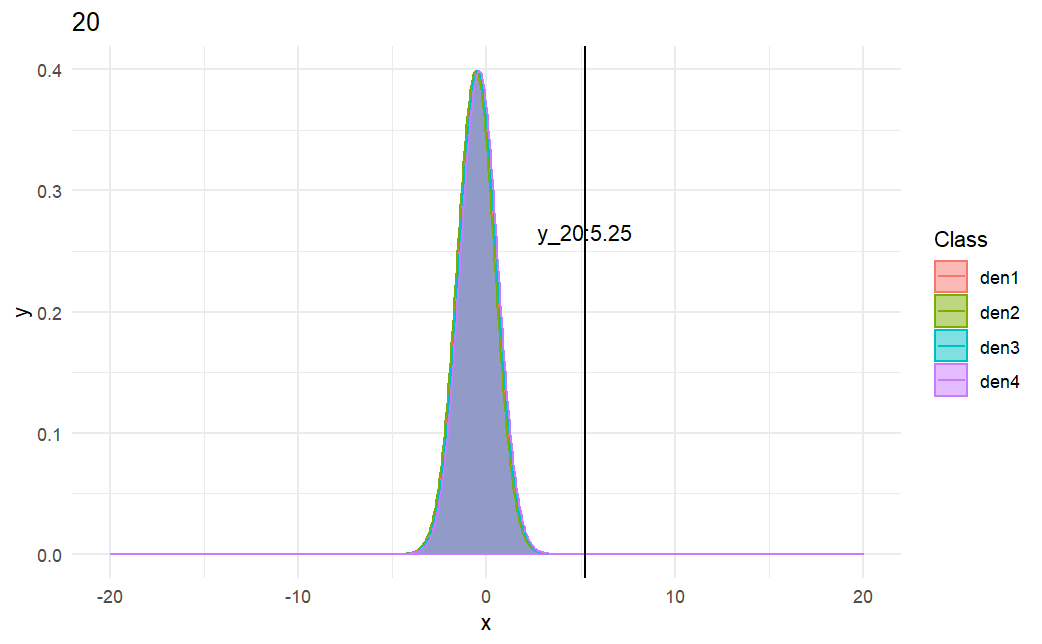
\includegraphics[width=2.7in]{img/test1-rhosame1.png}\\
			\vspace{0.02cm}
			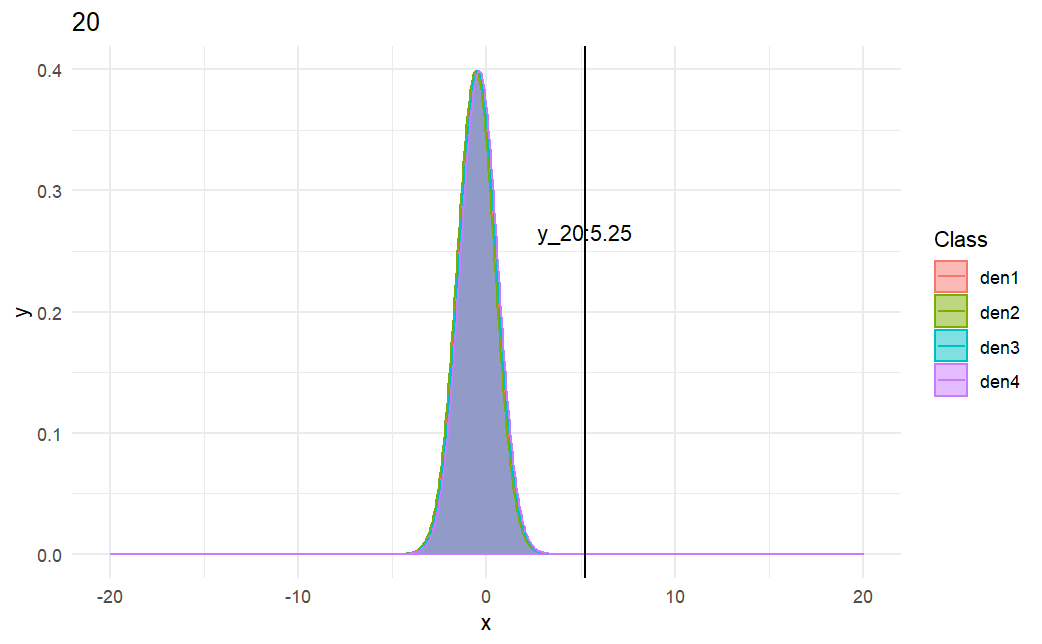
\includegraphics[width=2.7in]{img/test1-rhodiff1.png}\\
			\vspace{0.02cm}
		\end{minipage}%
	}%
	\subfigure{
	\begin{minipage}[t]{0.33\linewidth}
		\centering
		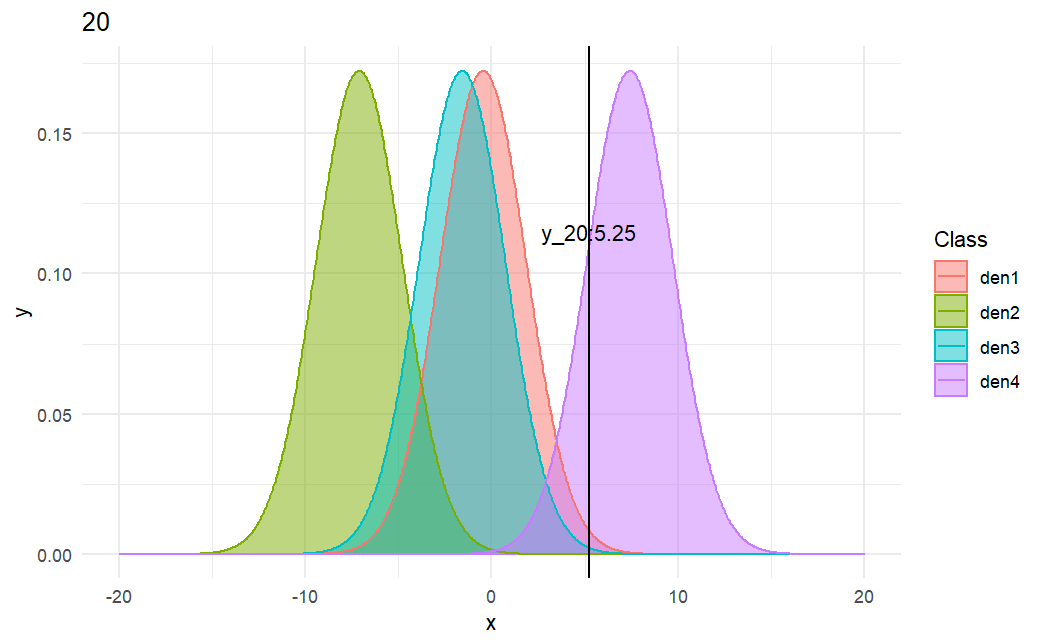
\includegraphics[width=2.7in]{img/test1-rhosame2.png}\\
		\vspace{0.02cm}
		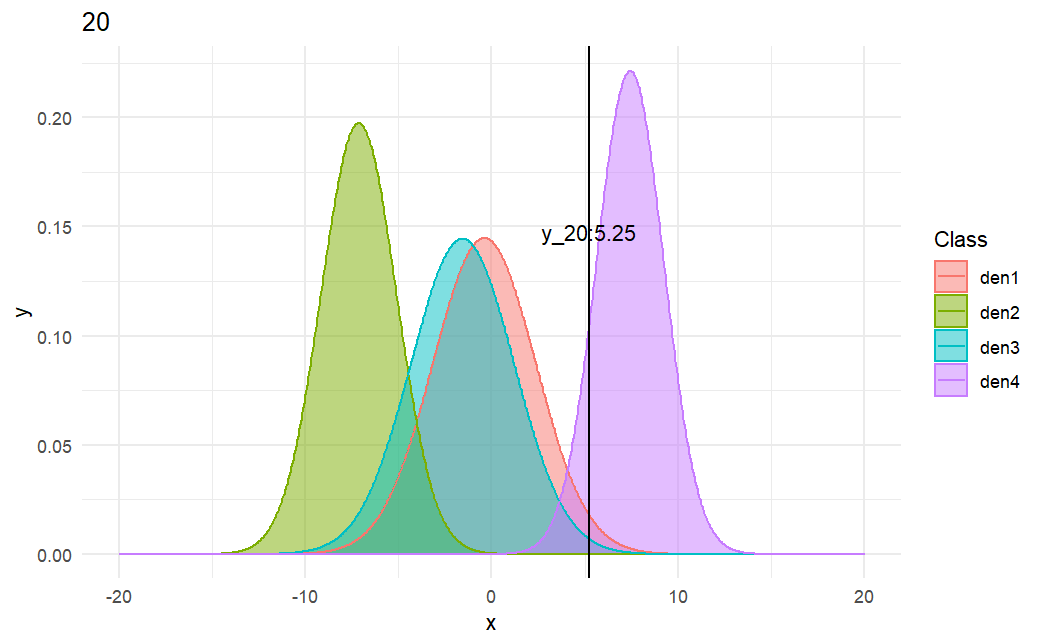
\includegraphics[width=2.7in]{img/test1-rhodiff2.png}\\
		\vspace{0.02cm}
	\end{minipage}%
	}%
	\subfigure{
	\begin{minipage}[t]{0.33\linewidth}
		\centering
		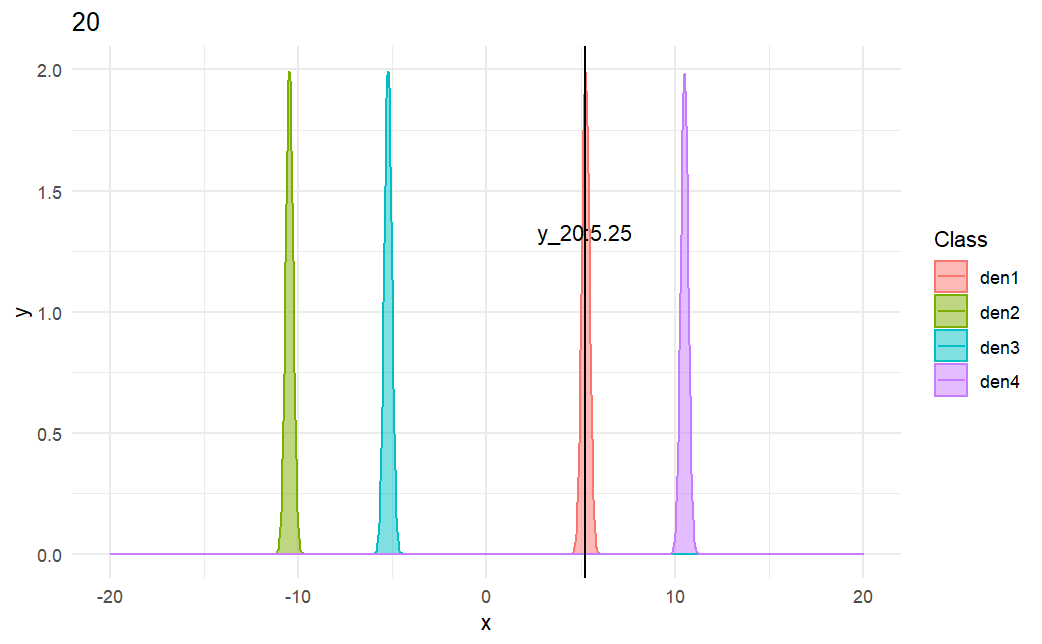
\includegraphics[width=2.7in]{img/test1-rhosame3.png}\\
		\vspace{0.02cm}
		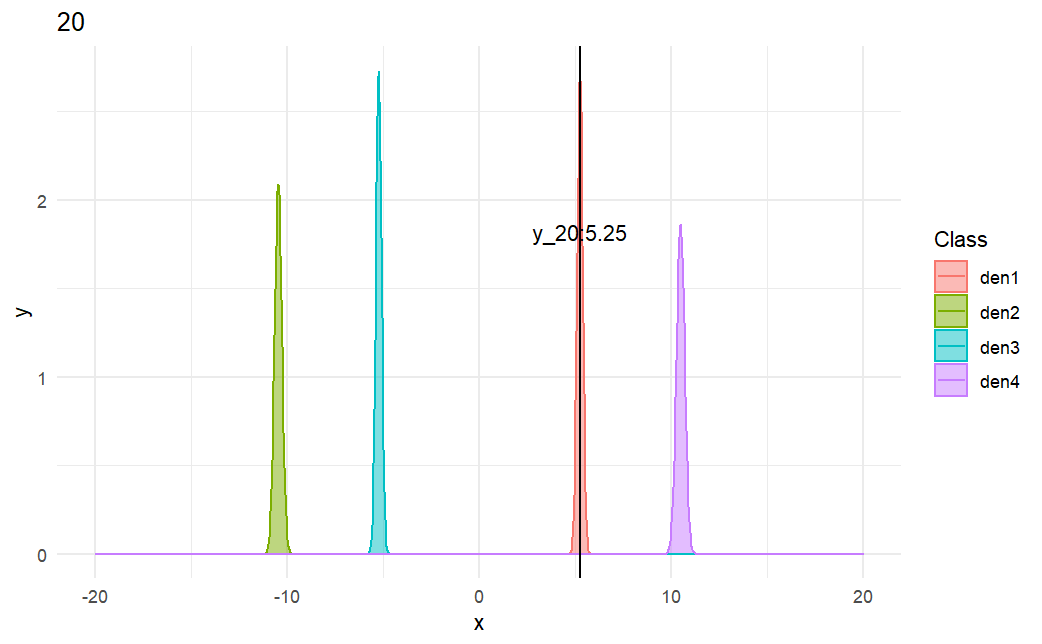
\includegraphics[width=2.7in]{img/test1-rhodiff3.png}\\
		\vspace{0.02cm}
	\end{minipage}%
	}%
	\centering
	\caption{简单设定下各类别分布随迭代轮数变化图(样本 20 为例,第一行为相同类别共用 $\rho$ 的设定,第二行为各类别分别更新各自 $\rho_k$ 的设定)}
	\vspace{-0.2cm}
	\label{fig:simple-vis}
\end{figure*}




\subsection{Simple Set2-Two Part}

\subsubsection{Estimation}

该部分本质上依旧是不包含交互项的多分类回归问题,在类别内部有

\begin{equation}
	Y_i = X_i^T\beta_k + Z_i^T\alpha_k, if\ i\in Class\ k
\end{equation}

其中 $\beta_k \in \mathbb{R}^p$,$\alpha_k \in \mathbb{R}^q$,若记 $\tilde X_i^T = (X_i^T, Z_i^T), \theta_k^T = (\beta_k^T, \alpha_k^T)$ 可以将模型改写为 $Y_i = \tilde X_i^T\theta_k$,此时完全退化为最简单线性设定,本部分的重点在于验证两部分依次各自更新迭代公式的正确性。

对于类别 $k$,可以对不同参数写出优化目标,计算时依次迭代即可。

\paragraph{Estimate $\beta_k$}

\begin{equation}
	\begin{aligned}
		\text{min}\qquad l_k &=  \displaystyle\sum_{i=1}^{n}q_{C_i}(k)\left(y_i - X_i^T \beta_k - Z_i^T \alpha_k\right) \\
		&= (y^{\beta_k} - X\beta_k)^T W_k (y^{\beta_k} - X\beta_k)
	\end{aligned}
\end{equation}

其中 $W_k = diag(q_{C_1}(k),...,q_{C_n}(k))$,则 $\beta_k$ 的估计值为

\begin{equation}
	\hat \beta_k = (X^{T} W_k X)^{-1} X^{T} W_k y^{\beta_k}
\end{equation}


\paragraph{Estimate $\alpha_k$}

\begin{equation}
	\begin{aligned}
		\text{min}\qquad l_k &=  \displaystyle\sum_{i=1}^{n}q_{C_i}(k)\left(y_i - X_i^T \beta_k - Z_i^T \alpha_k\right) \\
		&= (y^{\alpha_k} - Z\alpha_k)^T W_k (y^{\alpha_k} - Z\alpha_k)
	\end{aligned}
\end{equation}

$\alpha_k$ 的估计值为

\begin{equation}
	\hat \alpha_k = (Z^T W_k Z)^{-1}Z^T W_k y^{\alpha_k}
\end{equation}

值得注意的是,将两部分参数当做一体的方法更新公式 \ref{eq:two-part1} 与分别更新 $\beta_k,\alpha_k$ 的公式 \ref{eq:two-part2} 并不等价。公式 \ref{eq:two-part1} 中 $\beta_k$ 的更新不依赖于当前 $\alpha_k$ 的取值,反之亦反;而公式 \ref{eq:two-part2} 中 $y^{\beta_k} = y - Z\alpha_k,y^{\alpha_k} = y - X\beta_k$,$\beta_k$ 与 $\alpha_k$ 的更新相互依赖。直观理解上来看,二者计算目标不同,推导方法参照分块矩阵求逆。
\begin{equation}
	\left(\begin{array}{c}
		\hat{\beta}_{k} \\
		\hat{\alpha}_k
	\end{array}\right) = \left((X\ Z)^TW_k (X\ Z)\right)^{-1}(X\ Z)^T W_k y
\label{eq:two-part1}
\end{equation}

\begin{equation}
	\left\{\begin{array}{l}
		\hat{\beta}_{k}=  (X^{T} W_k X)^{-1} X^{T} W_k y^{\beta_k}\\
		\hat{\alpha}_{k}= (Z^T W_k Z)^{-1}Z^T W_k y^{\alpha_k}
	\end{array}\right.
	\label{eq:two-part2}
\end{equation}

\subsubsection{Numerical Setting}

令 $p=4,q=3$ 四个类别真实参数设置见表 \ref{tb:coef_true_twopart}

\begin{table}[h]
	\centering
	\caption{两部分参数设定}
	\begin{tabular}{ccccc}
		\toprule
		& Comp.1 & Comp.2 & Comp.3 & Comp.4 \\
		\midrule
		$\beta_{k1}$  & -2      & -1      & 1      & 2     \\
		$\beta_{k2}$  & -2      & -1      & 1      & 2     \\
		$\beta_{k3}$  & 0      & 0      & 0      & 0      \\
		$\beta_{k4}$  & 0      & 0      & 0      & 0      \\
		$\alpha_{k1}$  & -2      & -1      & 1      & 2      \\
		$\alpha_{k2}$  & -2      & -1      & 1      & 2      \\
		$\alpha_{k3}$  & 0      & 0      & 0      & 0      \\
		\bottomrule
	\end{tabular}
	\label{tb:coef_true_twopart}
\end{table}

\subsubsection{Results}

如果根据 $Y_i = \tilde X_i^T\theta_k$ 使用最简情况方法进行求解,可收敛,但初始值的设置需要比较小心。当初始值为一组来自 $N(0,0.1)$ 的随机数时候依旧很快(27轮左右)收敛到真值,但若抽样正态分布方差较大,会出现参数估计不再变化但未收敛到真值的情况。

%另外在实验中注意到,将两部分参数当做一体的迭代方法相较 $\beta_k, \alpha_k$ 分别更新的方法收敛较慢(不确定)










\subsection{Simple Set3-Interaction}

\subsubsection{Estimation}

以上为有分组的简单回归情况,现考虑原模型的协变量构成,即:$X,Z,W$(对应回归参数为 $\beta, \alpha, \eta$,其中 $\eta$ 又由 $\beta,\gamma$ 计算得到,真实需要更新的参数为 $\beta, \alpha, \gamma$),其中 $W$ 为交互项,$Z$ 为环境相关自变量,$X$ 为基因相关自变量。 
考虑加入交互项,目标函数 $\mu_{ik}$ 的成分发生变化,影响和 $\beta,\gamma$ 相关的求解。不影响 $\alpha$ 的求解。

与式 \ref{eq:l} 形式类似有

\begin{equation}
	\begin{aligned}
		l &= \displaystyle\sum_{i=1}^{n}\sum_{k=1}^{K}q_{C_i}(k)\left(C - \frac{\rho^2}{2}(y_i - \mu_{ik})^2 \right) \\
		&= \displaystyle\sum_{i=1}^{n}\sum_{k=1}^{K}q_{C_i}(k)\left(C - \frac{\rho^2}{2}(y_i - X_i^T \beta_k - Z_i^T \alpha_k - W_i^T \eta_k)^2 \right)
	\end{aligned}
\end{equation}

为了方便从交互项中按照不同需要拆分出系数,验证以下几种表达形式的等价(数值验证)

\begin{equation}
	\begin{aligned}
		W_i^T \eta_i &= W_i^T(I_q\otimes\beta_k \odot \gamma_k) \\
		&= \sum_{s=1}^{q}W_i^{(s)T}\beta_k\odot \gamma_{ks} \\
		&= (\sum_{s=1}^{q}W_i^{(s)}\odot \gamma_{ks})^T \beta_k \\
		&= (W_i \odot (I_q \otimes \beta_k))^T \gamma_k
	\end{aligned}
\label{eq:same}
\end{equation}

对于类别 $k$,可以对不同参数写出优化目标

\paragraph{Estimate $\alpha_k$}

\begin{equation}
	\begin{aligned}
		\text{min}\qquad l_k &=  \displaystyle\sum_{i=1}^{n}q_{C_i}(k)\left(y_i - X_i^T \beta_k - Z_i^T \alpha_k - W_i^T \eta_k\right) \\
		&= (y^{\alpha_k} - Z\alpha_k)^T W_k (y^{\alpha_k} - Z\alpha_k)
	\end{aligned}
\end{equation}

其中 $y_i^{\alpha_k} = y_i - X_i^T \beta_k - W_i^T \eta_k$, $y^{\alpha_k} = (y_1^{\alpha_k},...,y_n^{\alpha_k})^T$,$W_k = diag(q_{C_1}(k),...,q_{C_n}(k))$,则 $\alpha_k$ 的估计值为

\begin{equation}
	\hat \alpha_k = (Z^T W_k Z)^{-1}Z^T W_k y^{\alpha_k}
\end{equation}

\paragraph{Estimate $\beta_k$}

\begin{equation}
	\begin{aligned}
		\text{min}\qquad l_k &=  \displaystyle\sum_{i=1}^{n}q_{C_i}(k)\left(y_i - X_i^T \beta_k - Z_i^T \alpha_k - W_i^T \eta_k\right) \\
		&= (y^{\beta_k} - X^{\beta_k}\beta_k)^T W (y^{\beta_k} - X^{\beta_k}\beta_k)
	\end{aligned}
\end{equation}

其中 $X^{\beta_k} = (X^{\beta_k}_1,...,X^{\beta_k}_n)^T \in \mathbb{R}^{n\times p}$, $X^{\beta_k}_i = X_i + (\sum_{s=1}^{q}W_i^{(s)}\odot\gamma_{ks}) \in \mathbb{R}^{p\times 1}$, $y_i^{\beta_k} = y_i - Z_i^T\alpha_k, y_i^{\beta_k} = (y_1^{\beta_k},...,y_n^{\beta_k})^T$,$W_k = diag(q_{C_1}(k),...,q_{C_n}(k))$,则 $\beta_k$ 的估计值为

\begin{equation}
	\hat \beta_k = (X^{\beta_k T} W_k X^{\beta_k})^{-1} X^{\beta_k T} W_k y^{\beta_k}
\end{equation}

\paragraph{Estimate $\gamma_k$}

\begin{equation}
	\begin{aligned}
		\text{min}\qquad l_k &=  \displaystyle\sum_{i=1}^{n}q_{C_i}(k)\left(y_i - X_i^T \beta_k - Z_i^T \alpha_k - W_i^T \eta_k\right) \\
		&= (y^{\gamma_k} - X^{\gamma_k}\gamma_k)^T W (y^{\gamma_k} -  X^{\gamma_k}\gamma_k)
	\end{aligned}
\end{equation}

其中 $X^{\gamma_k} = (X^{\gamma_k}_1,...,X^{\gamma_k}_n)^T \in \mathbb{R}^{n\times pq}$, $X^{\gamma_k}_i = W_i\odot (I_q \otimes \beta_k) \in \mathbb{R}^{pq\times 1}$, $y_i^{\gamma_k} = y_i - X_i^T\beta_k - Z_i^T\alpha_k, y_i^{\gamma_k} = (y_1^{\gamma_k},...,y_n^{\gamma_k})^T$,$W_k = diag(q_{C_1}(k),...,q_{C_n}(k))$,则 $\gamma_k$ 的估计值为

\begin{equation}
	\hat \gamma_k = (X^{\gamma_k T} W_k X^{\gamma_k})^{-1} X^{\gamma_k T} W_k y^{\gamma_k}
\end{equation} 

$X^{\beta_k}$ 依赖于当前 $\gamma_k$ 估计值,$X^{\gamma_k}$ 也依赖于当前 $\beta_k$ 的估计值。有交互项的情况不再可以直接化为最简单的线性回归情况,即不可以一次性算出一轮参数的更新。综上,更新总结如式 \ref{eq:interaction}


\begin{equation}
	\left\{\begin{array}{l}
		\hat{\beta}_{k} = (X^{\beta_k T} W_k X)^{-1} X^{\beta_k T} W_k y^{\beta_k}\\
		\hat{\alpha}_{k} = (Z^T W_k Z)^{-1}Z^T W_k y^{\alpha_k}\\
		\hat{\gamma}_{k} = (X^{\gamma_k T} W_k X)^{-1} X^{\gamma_k T} W_k y^{\gamma_k}
	\end{array}\right.
	\label{eq:interaction}
\end{equation}

\subsubsection{Numerical Setting}

1. 主要实验设置:$p=4,q=3,n=200,K=4$,真实参数设置如表 \ref{tb:coef_true} 

2. 辅助实验设置:$p=2,q=2,n=200,K=4$,真实参数设置如表 \ref{tb:coef_true} 中非零项

\subsubsection{Package Results}

注意在有交互项的模型中,包得到的结果和上述更新不同。形式 

\begin{equation}
	\begin{aligned}
		y_i &= \displaystyle\sum_{k=1}^{K} q_{C_i}(k) \left(X_i^T \beta_k + Z_i^T \alpha_k + W_i^T \eta_k\right) \\
		&= \displaystyle\sum_{k=1}^{K} q_{C_i}(k) \left(X_i^T \beta_k + Z_i^T \alpha_k + (W_i \odot (I_q \otimes \beta_k))^T \gamma_k\right)
	\end{aligned}
\end{equation}

加权最小二乘法得到的是 $\beta_k, \alpha_k, \gamma_k$ 的更新,$\eta_k$ 是根据其他参数计算出来的。而直接用包得到的参数为 $\beta_k, \alpha_k, \eta_k$, $\gamma_k$ 需要再计算。当然也可以重新定义 $\gamma_k$ 相关的自变量为 $W_i \odot (I_q \otimes \beta_k)$,但该表达式包含 $\beta_k$。

\textit{fmrs}:$p=2,q=2$ 效果不好

\textit{flexmix}:$p=2,q=2$ 计算正确

\begin{table}[h]
	\centering
	\begin{tabular}{ccccc}
		\toprule
		& Comp.1 & Comp.2 & Comp.3 & Comp.4 \\
		\midrule
		$\beta_{k1}$   & 2      & 2      & -2     & -2     \\
		$\beta_{k2}$   & 2      & 2      & -2     & -2     \\
		$\beta_{k3}$   & 0      & 0      & 0      & 0      \\
		$\beta_{k4}$   & 0      & 0      & 0      & 0      \\
		\midrule
		$\alpha_{k1}$  & 2      & 2      & -2     & -2     \\
		$\alpha_{k2}$  & 2      & 2      & -2     & -2     \\
		$\alpha_{k3}$  & 0      & 0      & 0      & 0      \\
		\midrule
		$\gamma_{k1}$  & 3      & 1      & -1     & -3     \\
		$\gamma_{k2}$  & 3      & 1      & -1     & -3     \\
		$\gamma_{k3}$  & 3      & 1      & -1     & -3     \\
		$\gamma_{k4}$  & 3      & 1      & -1     & -3     \\
		$\gamma_{k5}$  & 0      & 0      & 0      & 0      \\
		$\gamma_{k6}$  & 0      & 0      & 0      & 0      \\
		$\gamma_{k7}$  & 0      & 0      & 0      & 0      \\
		$\gamma_{k8}$  & 0      & 0      & 0      & 0      \\
		$\gamma_{k9}$  & 0      & 0      & 0      & 0      \\
		$\gamma_{k10}$ & 0      & 0      & 0      & 0      \\
		$\gamma_{k11}$ & 0      & 0      & 0      & 0      \\
		$\gamma_{k12}$ & 0      & 0      & 0      & 0     \\
		\bottomrule
	\end{tabular}
	\label{tb:coef_true}
\end{table}

直接计算流程类似于算法 \ref{alg:simplest},固定其他参数依次更新 $\beta_k, \alpha_k, \gamma_k$ 即可。

\subsubsection{Iteration Results}

直接计算算法不收敛且距离真值越来越远,为了检测问题所在,进行固定部分参数,只迭代剩余参数的实验,参数距离真值的距离随迭代步数变化情况如图 \ref{fig:split1} 所示,图片标题表示用于迭代的参数。

\begin{figure*}
	\centering
	\subfigure{
		\begin{minipage}[t]{0.5\linewidth}
			\centering
			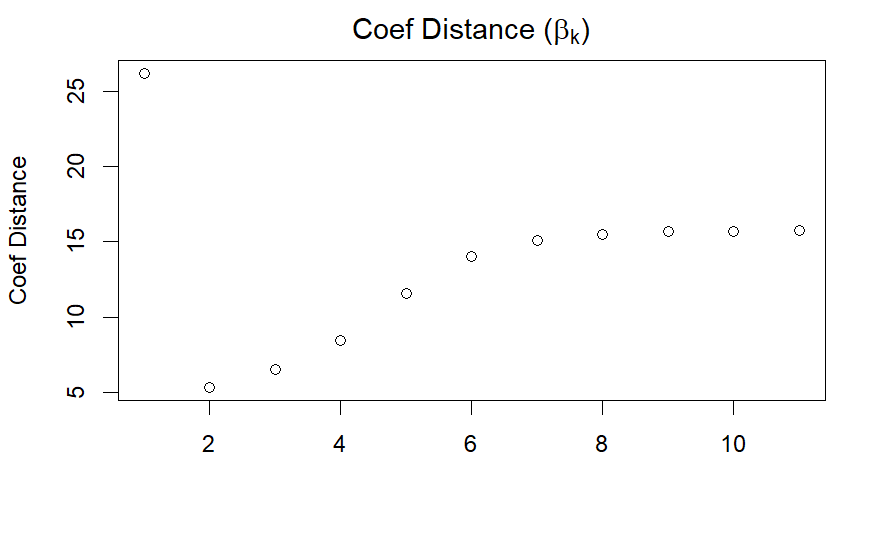
\includegraphics[width=3.5in]{img/split_only_beta.png}\\
			\vspace{0.02cm}
			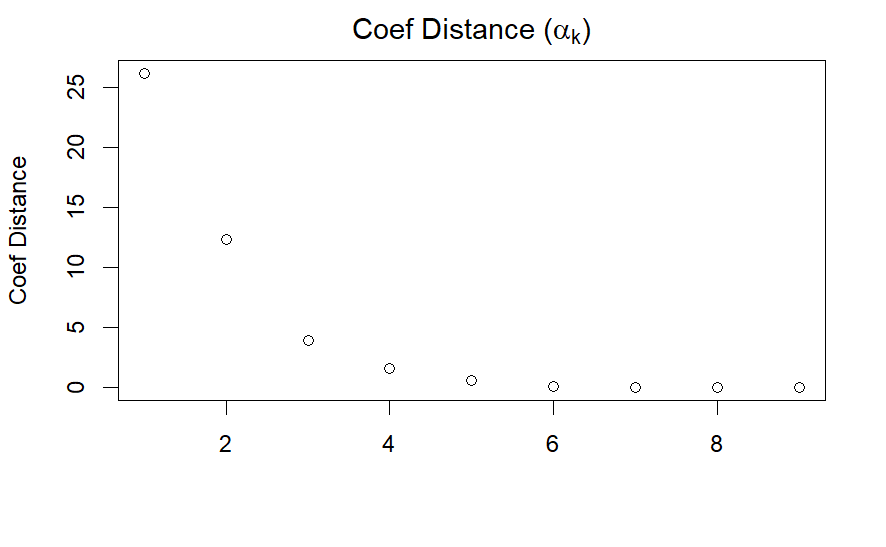
\includegraphics[width=3.5in]{img/split_only_alpha.png}\\
			\vspace{0.02cm}
			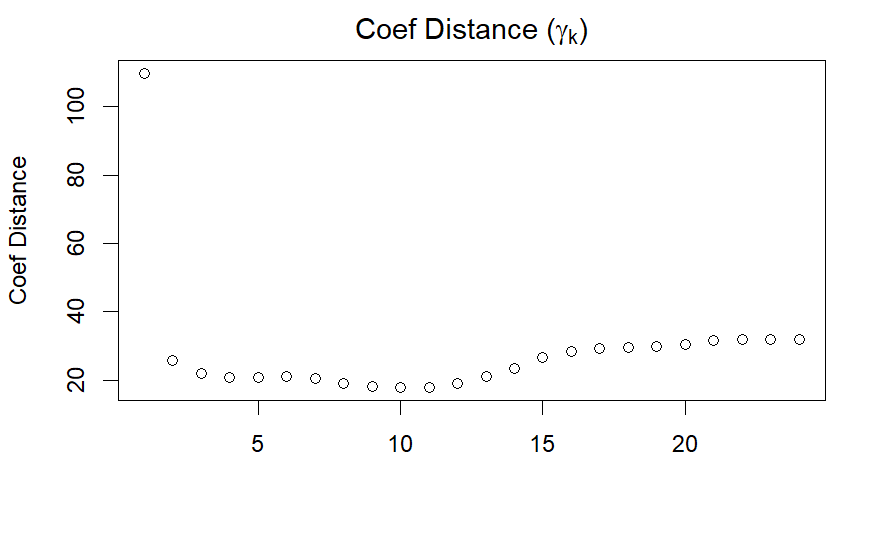
\includegraphics[width=3.5in]{img/split_only_gamma.png}\\
		\end{minipage}%
	}%
		\subfigure{
		\begin{minipage}[t]{0.5\linewidth}
			\centering
			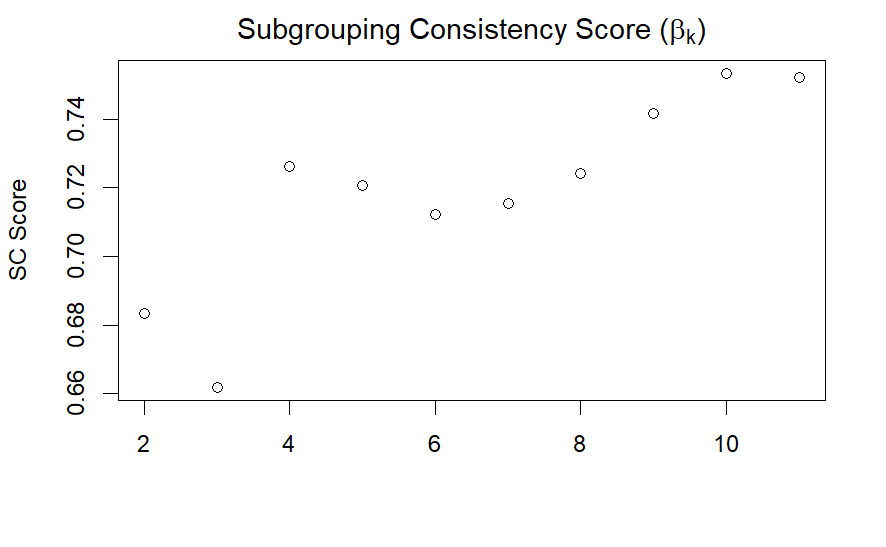
\includegraphics[width=3.5in]{img/split_only_beta_sc.png}\\
			\vspace{0.02cm}
			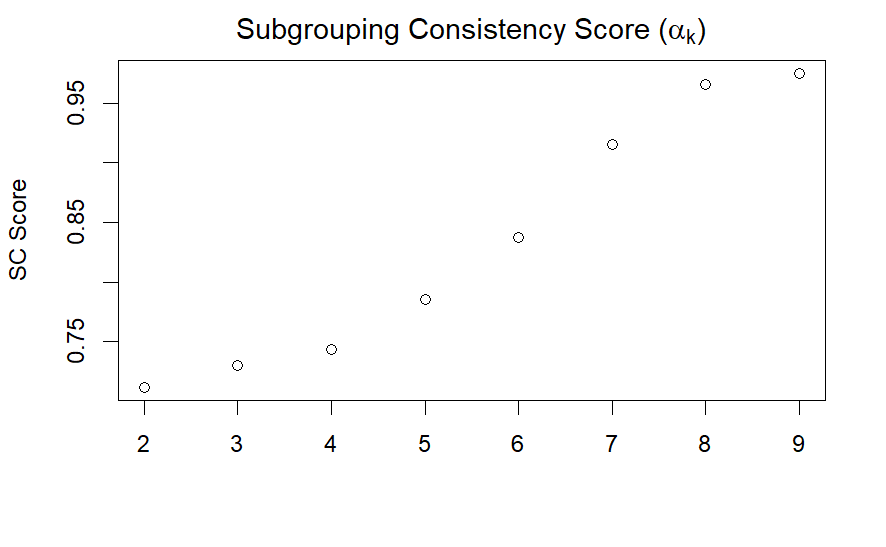
\includegraphics[width=3.5in]{img/split_only_alpha_sc.png}\\
			\vspace{0.02cm}
			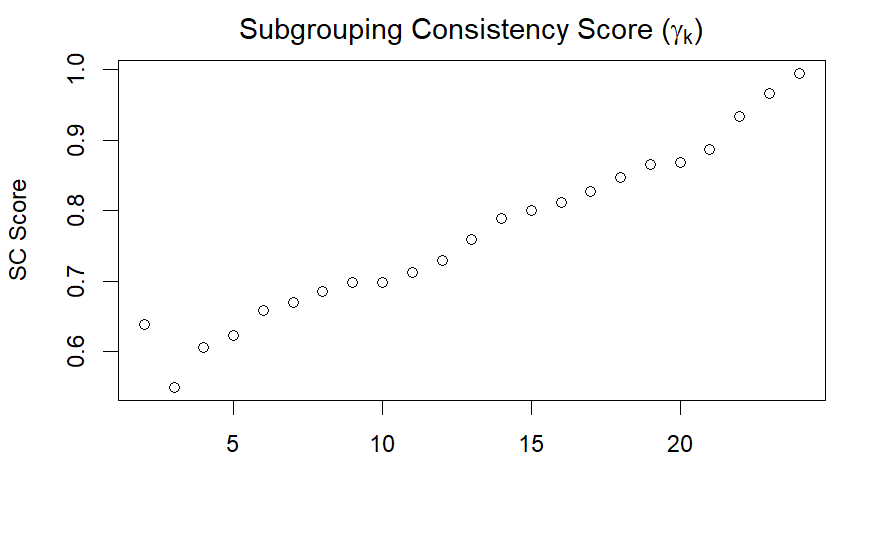
\includegraphics[width=3.5in]{img/split_only_gamma_sc.png}\\
		\end{minipage}%
	}%
	\centering
	\caption{包含交互项模型中更新单个参数,参数距离真值随迭代轮数变化示意图(子图标题表示用于迭代的参数)}
	\vspace{-0.2cm}
	\label{fig:split1}
\end{figure*}

\begin{figure*}
	\centering
	\subfigure{
		\begin{minipage}[t]{0.5\linewidth}
			\centering
			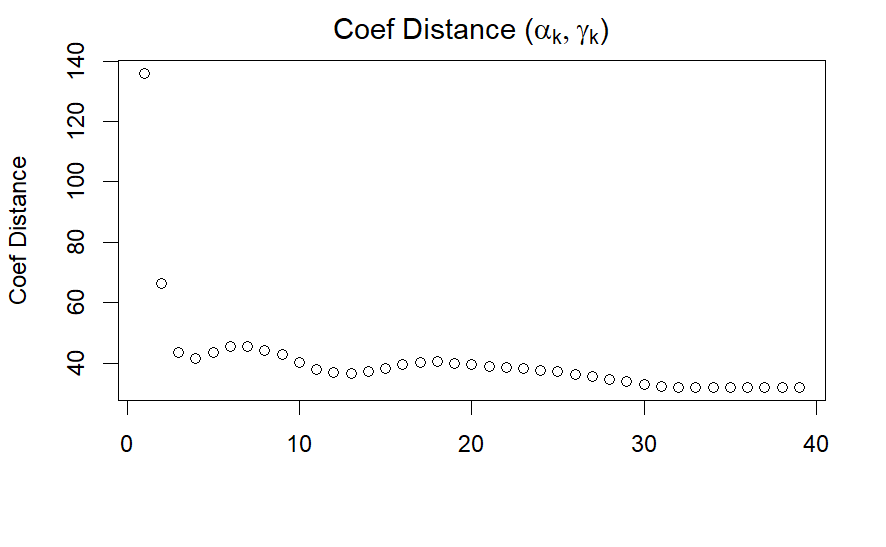
\includegraphics[width=3.5in]{img/split_except_beta.png}\\
			\vspace{0.02cm}
			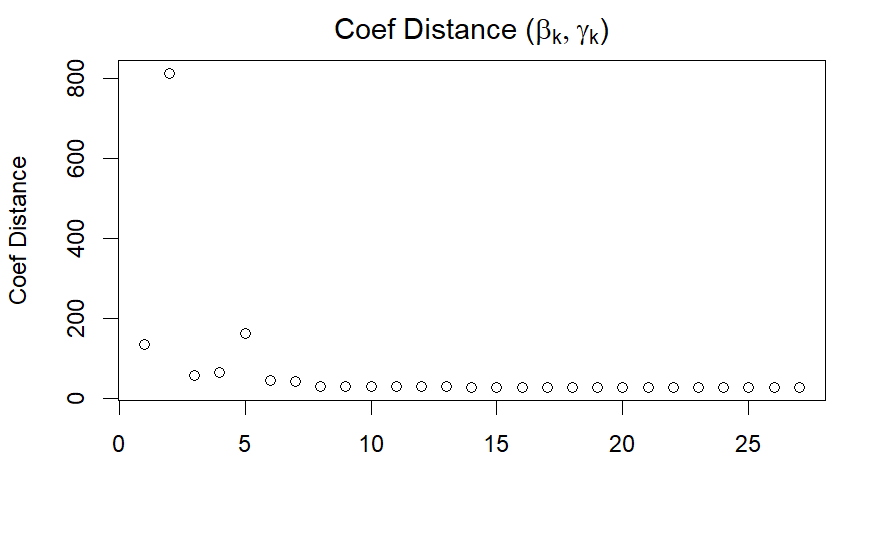
\includegraphics[width=3.5in]{img/split_except_alpha.png}\\
			\vspace{0.02cm}
			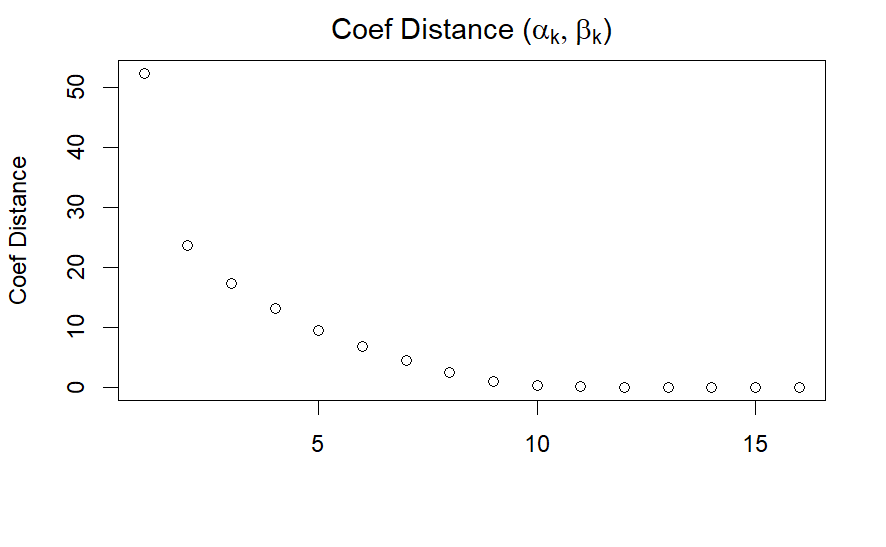
\includegraphics[width=3.5in]{img/split_except_gamma.png}\\
		\end{minipage}%
	}%
	\subfigure{
		\begin{minipage}[t]{0.5\linewidth}
			\centering
			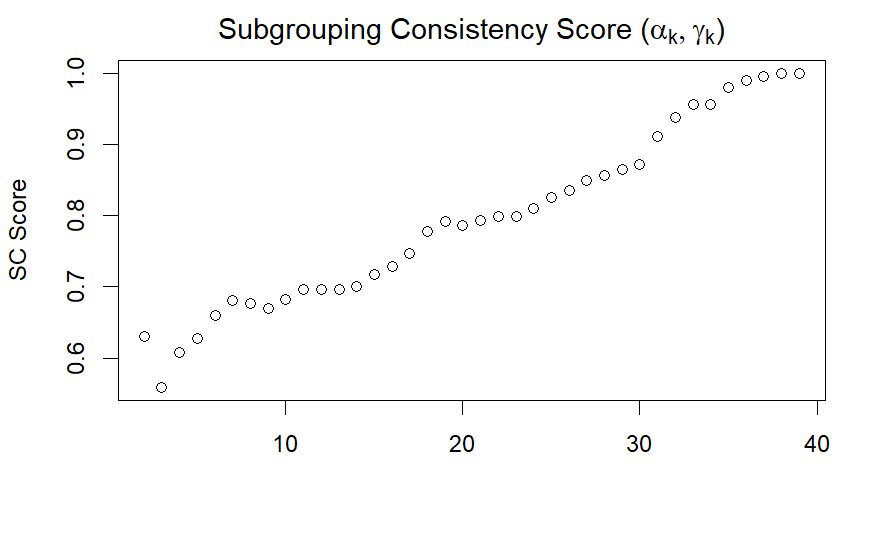
\includegraphics[width=3.5in]{img/split_except_beta_sc.png}\\
			\vspace{0.02cm}
			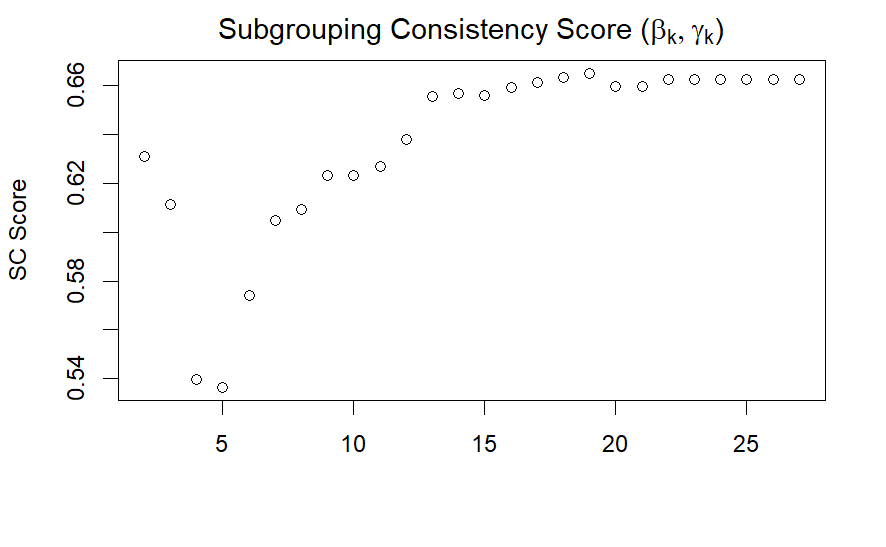
\includegraphics[width=3.5in]{img/split_except_alpha_sc.png}\\
			\vspace{0.02cm}
			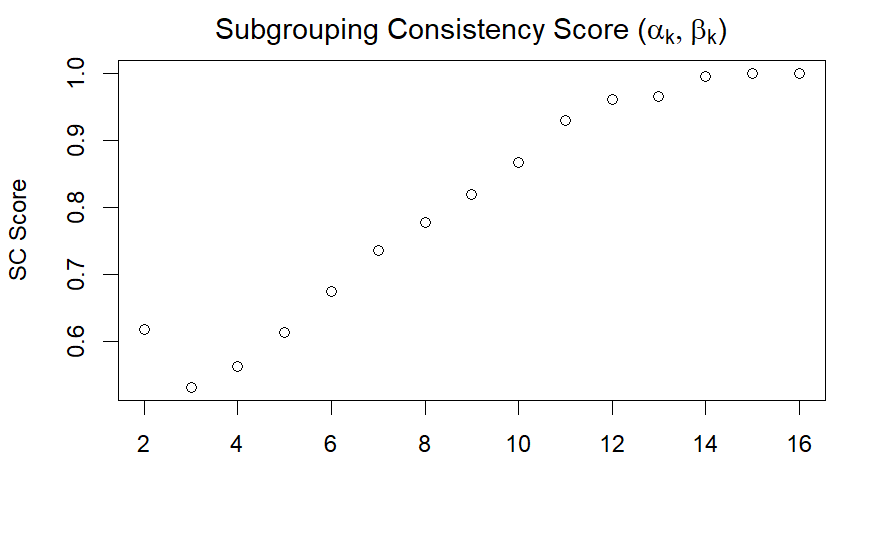
\includegraphics[width=3.5in]{img/split_except_gamma_sc.png}\\
		\end{minipage}%
	}%
	\centering
	\caption{包含交互项模型中更新多个参数,参数距离真值随迭代轮数变化示意图(子图标题表示用于迭代的参数)}
	\vspace{-0.2cm}
	\label{fig:split2}
\end{figure*}


\begin{figure*}
	\centering
	\subfigure{
		\begin{minipage}[t]{0.5\linewidth}
			\centering
			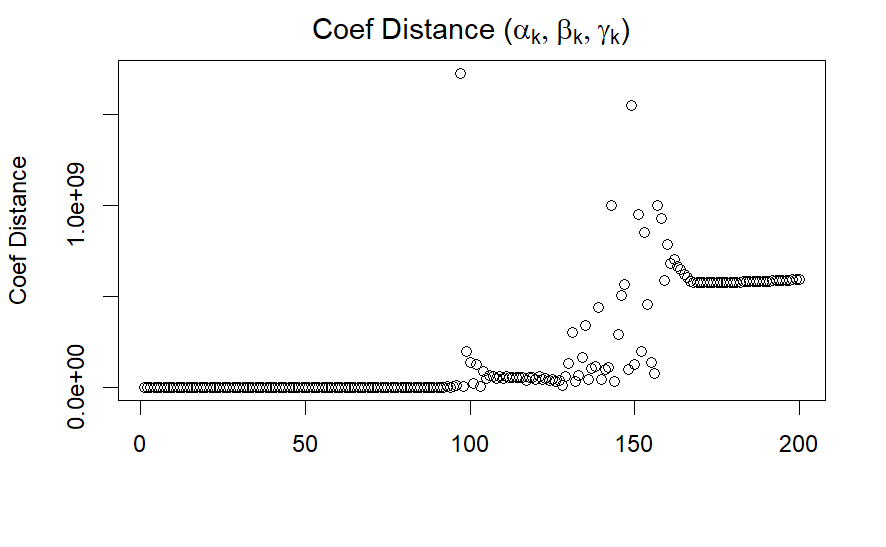
\includegraphics[width=3.5in]{img/split_all.png}\\
			\vspace{0.02cm}
			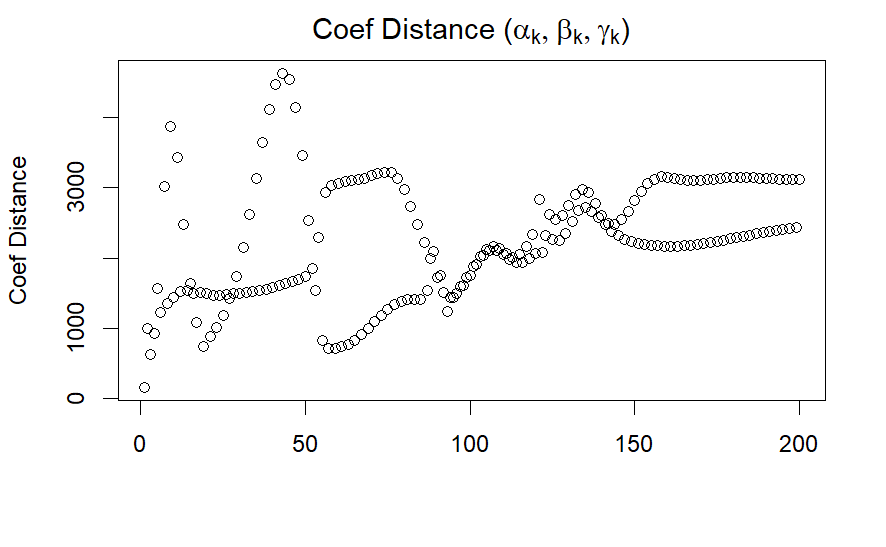
\includegraphics[width=3.5in]{img/split_all_add.png}\\
		\end{minipage}%
	}%
	\subfigure{
		\begin{minipage}[t]{0.5\linewidth}
			\centering
			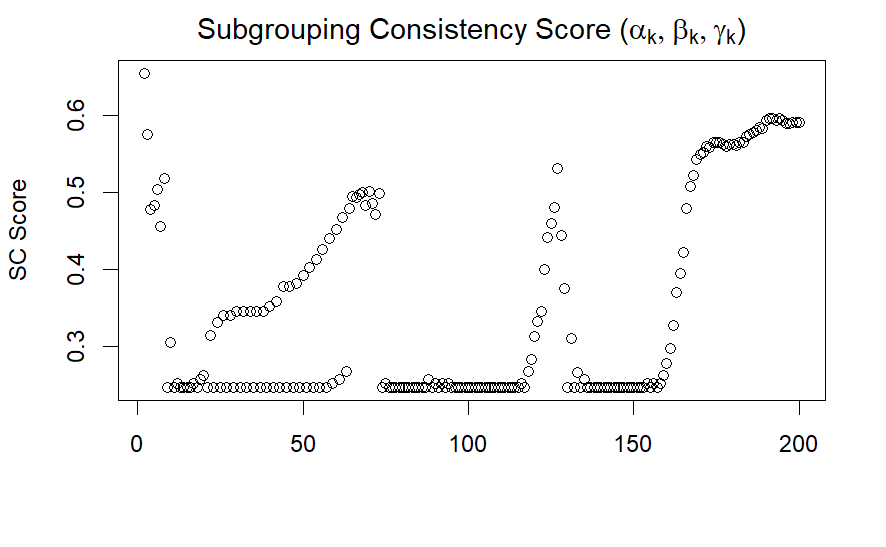
\includegraphics[width=3.5in]{img/split_all_sc.png}\\
			\vspace{0.02cm}
			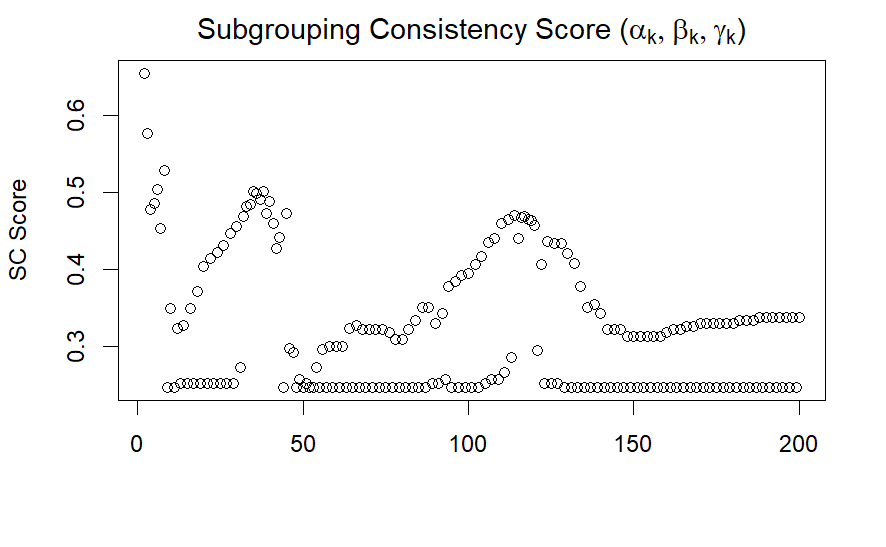
\includegraphics[width=3.5in]{img/split_all_add_sc.png}\\
		\end{minipage}%
	}%
	\centering
	\caption{包含交互项模型中更新多个参数,参数距离真值随迭代轮数变化示意图(子图标题表示用于迭代的参数)}
	\vspace{-0.2cm}
	\label{fig:split3}
\end{figure*}

从图 \ref{fig:split1} 中可以看到更新单个参数的所有情况都会收敛,单独更新 $\alpha_k$ 收敛且收敛到真值;单独更新 $\beta_k$ 收敛,未收敛到真值,但分类正确率总体上升;单独更新 $\gamma_k$ 收敛且收敛到真值,其与真值距离保持在 20 是因为只考虑 $\alpha_k, \beta_k$ 时只有两种分类,$\gamma_k$ 标记着更细致的分类,由 $\alpha_k, \beta_k$ 分出的第一大类的第一第二小类位置不固定,实际收敛到真值。

从图 \ref{fig:split2} 中可以看到更新两个参数的所有情况都会收敛。只更新 $\alpha_k, \gamma_k$ 收敛到非常接近真值的地方,分类得分达到 1;和只更新 $\beta_k, \gamma_k$ 的情况收敛到接近真值的地方,分类得分虽然呈上升趋势但局限于 0.68;只更新 $\alpha_k, \beta_k$ 的情况收敛效果不好,稳定在与真值相差较远的地方,分类得分约为 0.5;更新所有参数情况不收敛,分类得分随迭代次数有比较奇怪的周期性。

从图 \ref{fig:split3} 更新所有参数时,算法不收敛,分类得分和距离真实参数的距离变化都有比较奇怪的周期性。经检验发现取逆的矩阵特征值有较小的情况,如 0.002。图 \ref{fig:split3} 第一行为取逆项不加 $0.1 \times$ 对角阵结果,第二行为取逆项加 $0.1 \times$ 对角阵结果,结果不相同,在之前只更新部分参数的实验中加入该项影响很小。


\paragraph{更新单个参数 $\beta_k$ 详细信息}

只更新 $\alpha_k$ 实际为很纯粹的线性回归问题,完全退化为 \ref{subsec:test-set1};只更新 $\gamma_k$ 以及只更新 $\beta_k$ 的情况经过重写交互项形式不可完全退化为简单线性回归形式,因为 $y^{\beta_k}, y^{\gamma_k}, X^{\beta_k}, X^{\gamma_k}$ 在不同类别中不同($y^{\alpha_k}, X^{\alpha_k}$ 在各个类别中均相同,不同类别的参数更新依靠 $q_{C_i}$ 加以区分)。

在只更新 $\beta_k$ 而固定 $\alpha_k, \gamma_k$ 时,模型写为 \ref{eq:beta_test}

\begin{equation}
	\begin{aligned}
		y_i^{\beta_k} &= X_i^{\beta_k T} \beta_k \\
		y_i - Z_i \alpha_k &= \left(X_i + (\sum_{s=1}^{q}W_i^{(s)}\odot\gamma_{ks}) \right)^T \beta_k
	\end{aligned}
\label{eq:beta_test}
\end{equation} 

固定 $\alpha_k, \gamma_k$ 为真值,则在各个类别中 $y_i - Z_i \alpha_k, X_i + (\sum_{s=1}^{q}W_i^{(s)}\odot\gamma_{ks})$ 均为固定值,同样也是简单线性回归形式。依据之前推导,$\hat{\beta}_{k} = (X^{\beta_k T} W_k X)^{-1} X^{\beta_k T} W_k y^{\beta_k}$,这里 $W_k = diag(q_{C_1}(k),...,q_{C_n}(k))$. 依照上式进行更新,三步迭代即收敛,虽没有收敛到真值,但分类结果较为合理,使用不同方差的正态分布随机数对 $\beta_k$ 进行初始化结果如图 \ref{fig:heat-beta} 所示,$\beta_k$ 真值为表 \ref{tb:coef_true} 中相应部分的非零值,分类实际为两类。


\begin{figure}
	\centering
	\subfigure[$N(0,1)$初始化]{
		\begin{minipage}[t]{0.5\linewidth}
			\centering
			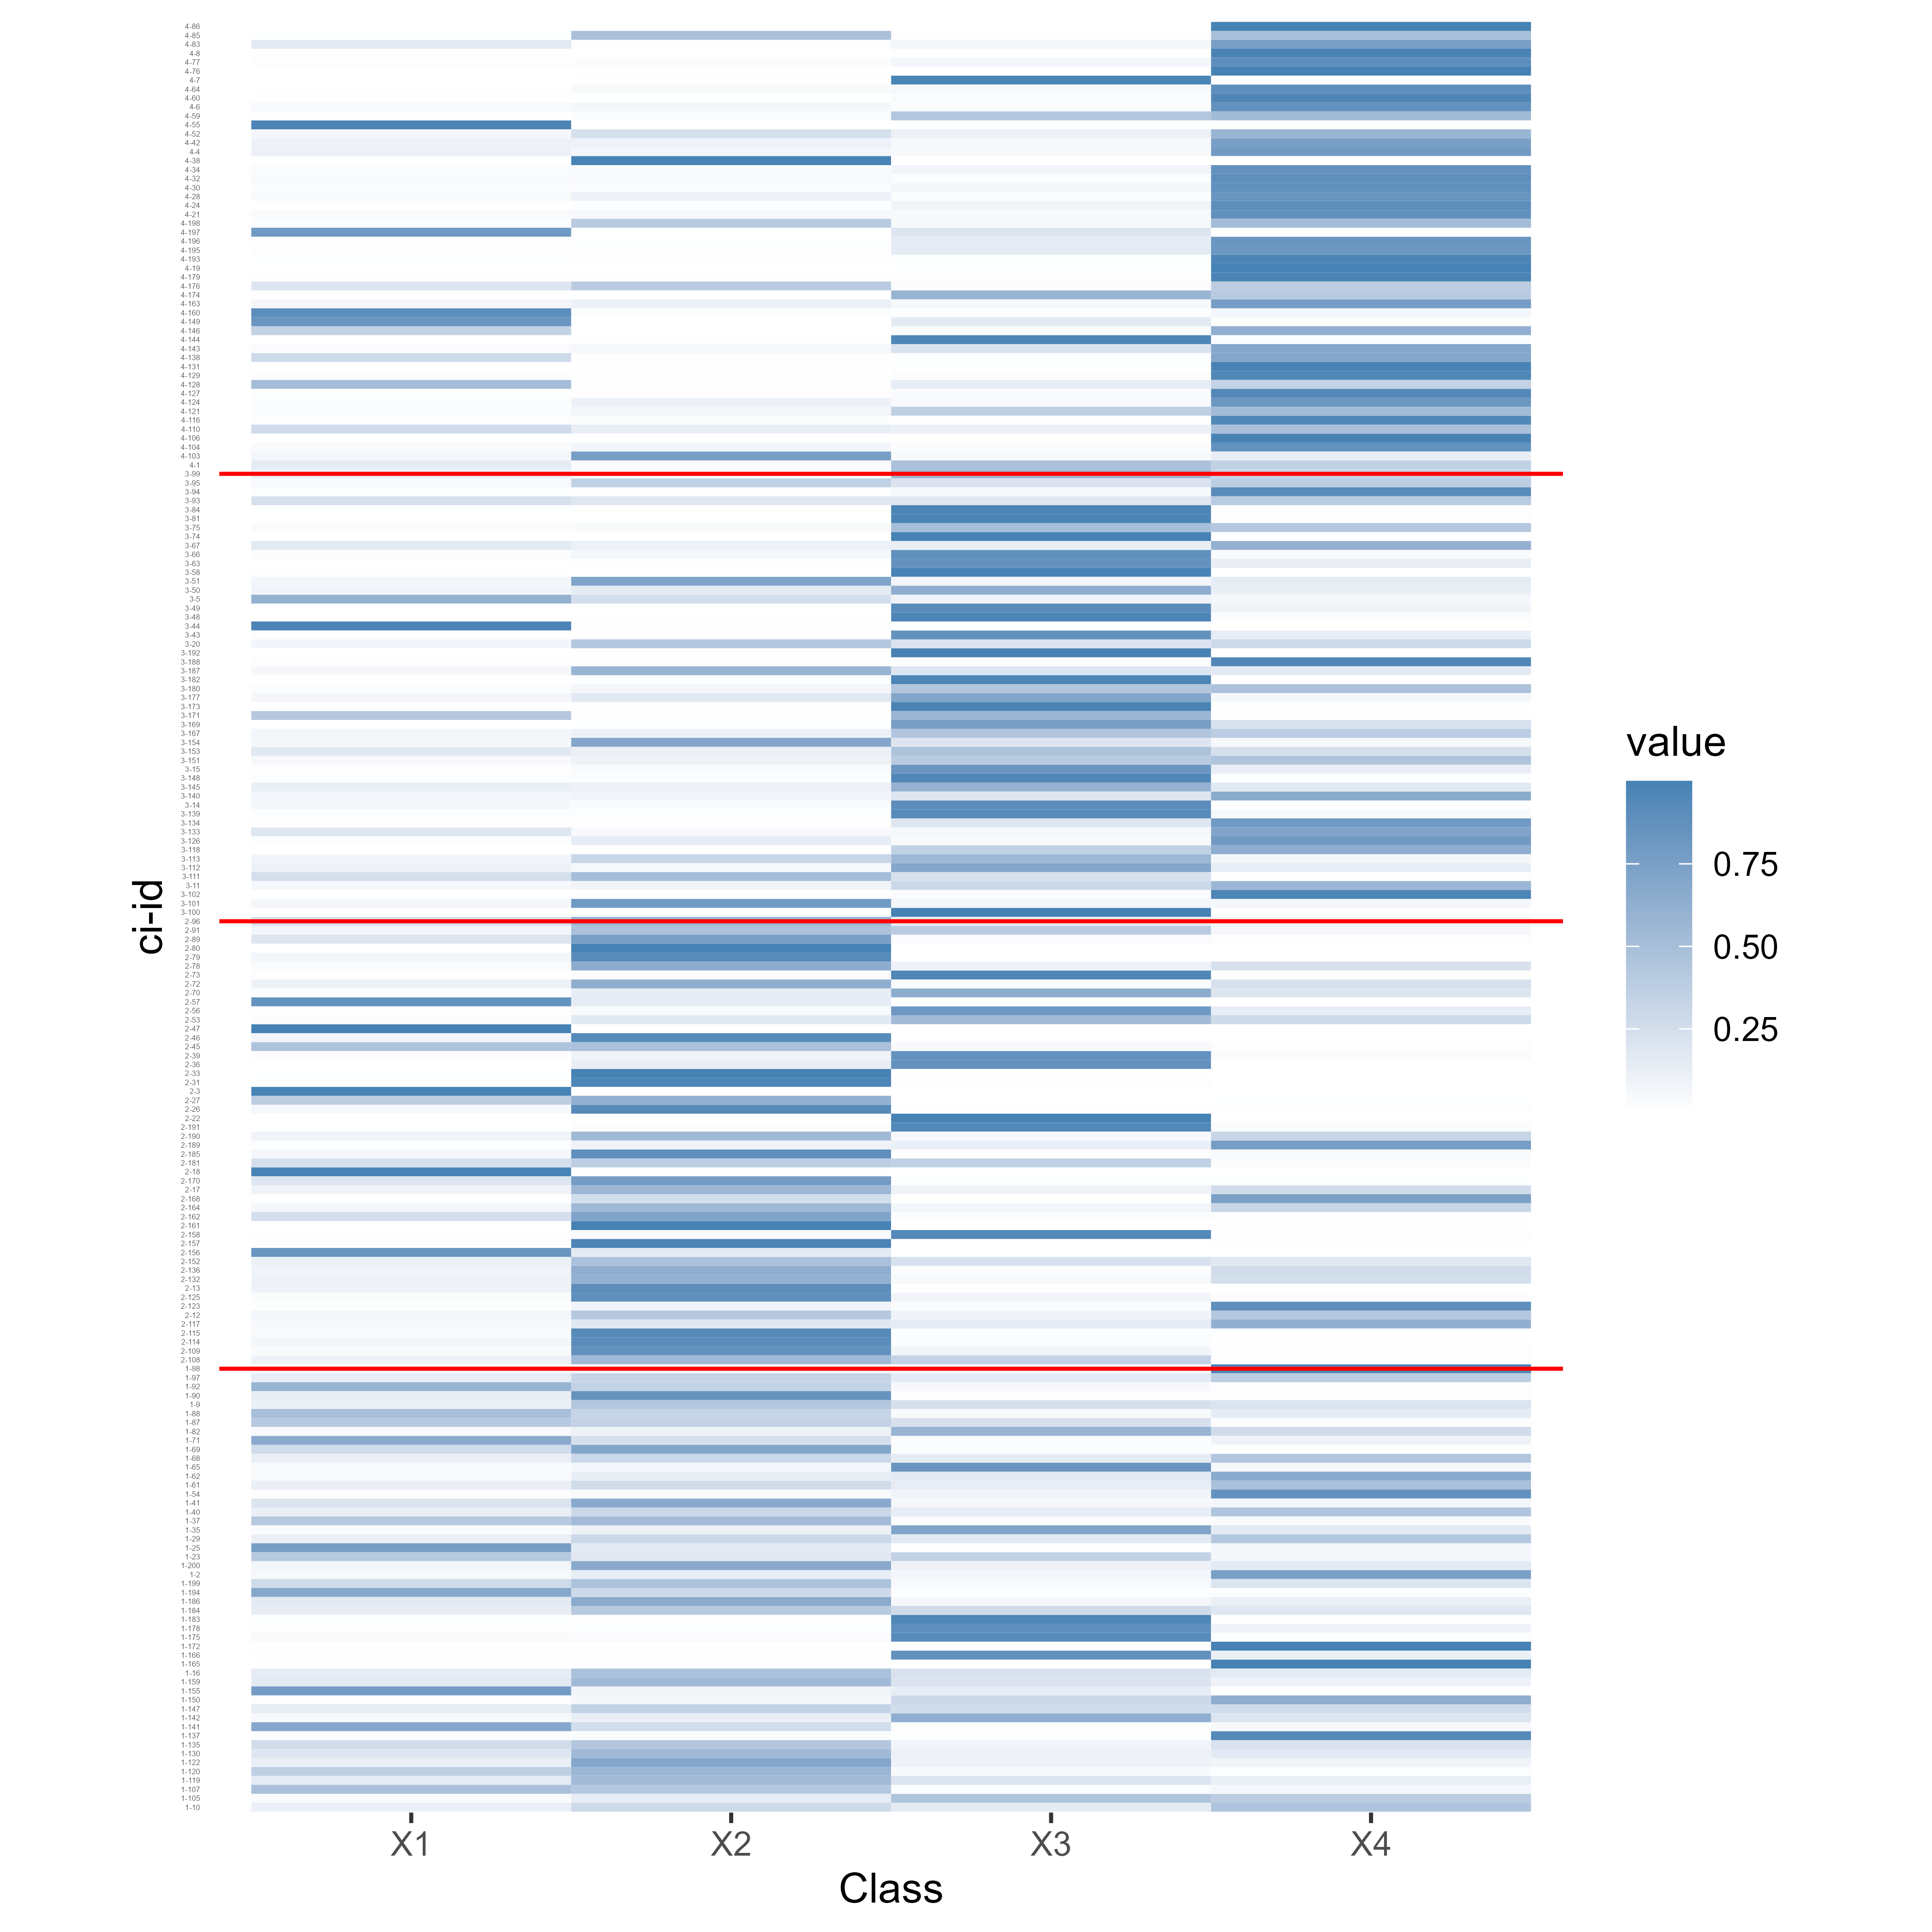
\includegraphics[width=3.5in]{img/q_c_beta.png}
		\end{minipage}%
	}%
	\subfigure[$N(0,4)$初始化]{
		\begin{minipage}[t]{0.5\linewidth}
			\centering
			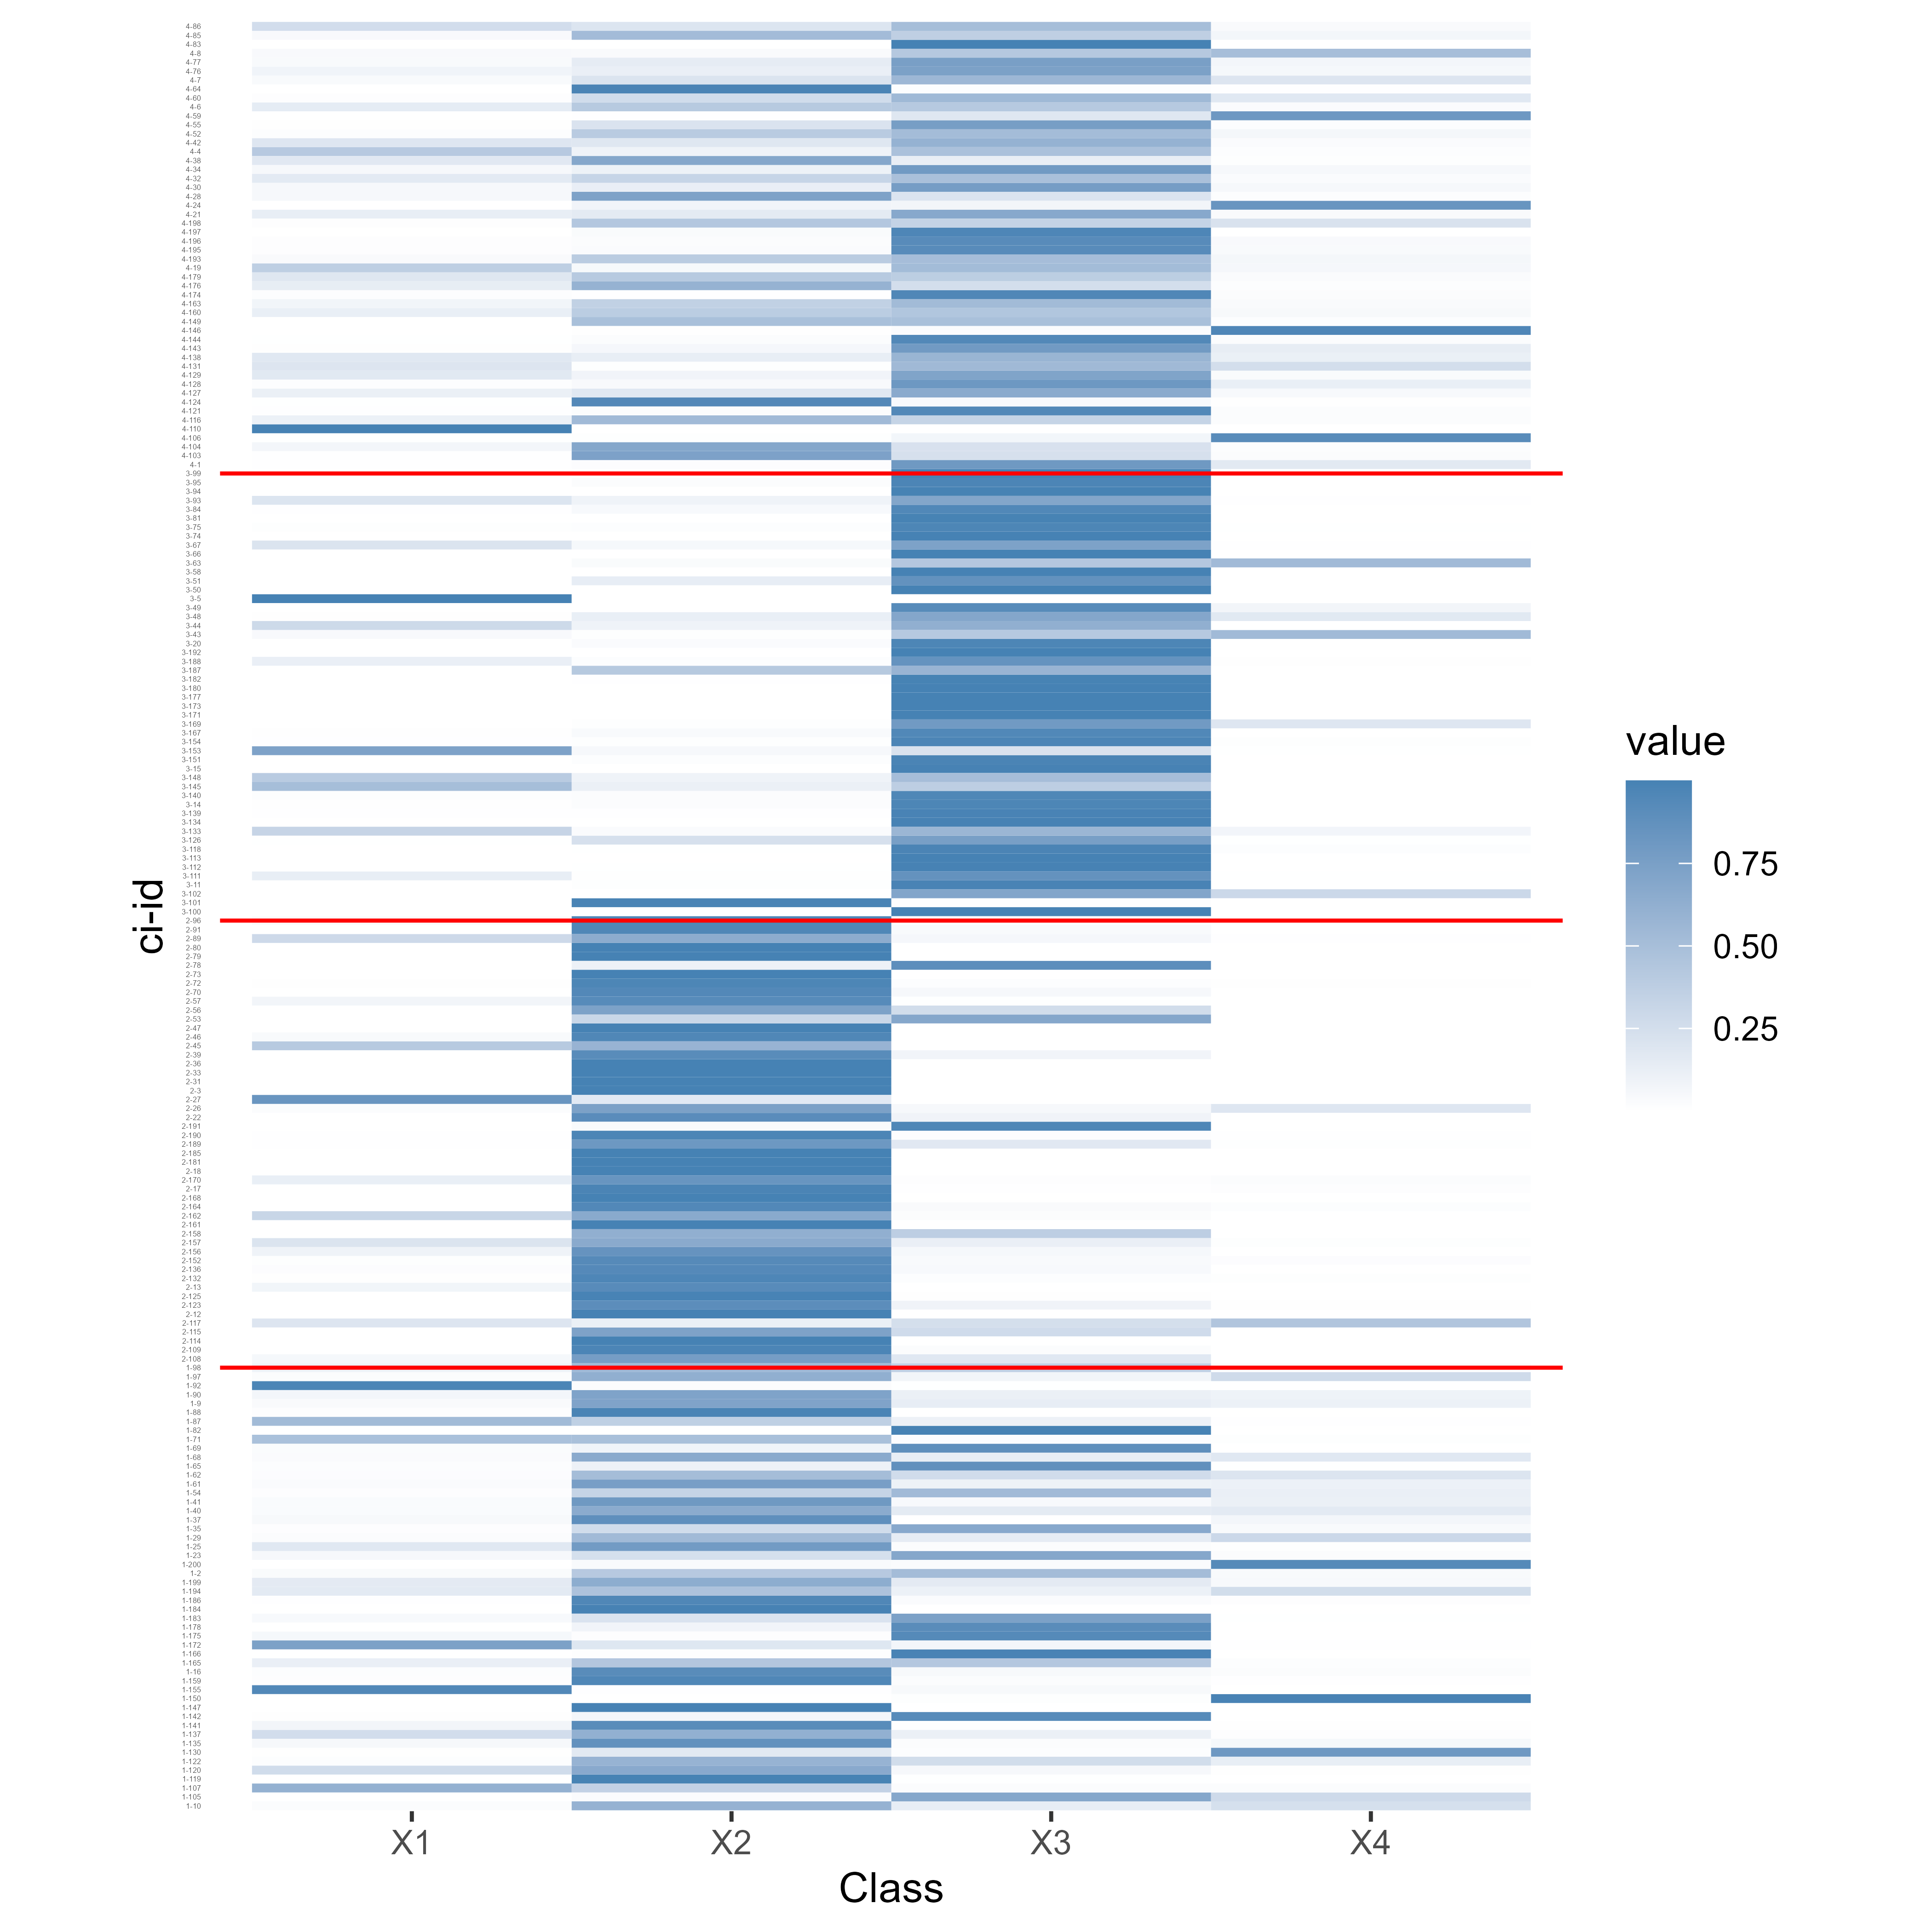
\includegraphics[width=3.5in]{img/q_c_beta2.png}\\
		\end{minipage}%
	}%
	\caption{单独更新 $\beta_k$ 情况收敛后后验概率分布图}
	\label{fig:heat-beta}
\end{figure}


\subsubsection{Test Detail}

\paragraph{单类检测}

测试如果只有一个分类(50 个样本,2+2+4 个待计算参数),依次迭代 $\alpha_k, \beta_k, \gamma_k$ 检查参数更新流程自身是否有有误。结论:单独更新参数没有问题;更新 $\alpha_k, \beta_k$ 或 更新 $\alpha_k, \gamma_k$ 时十几次迭代后更新到真值($N(0,1)$ 随机初始化)。使用上一轮结果更新 $\beta_k, \gamma_k$ 时无法收敛,参数距离真值的距离有很强且有规律的跳跃性,如图 \ref{fig:beta-gamma-jump};但若实时使用最新 $\beta_k, \gamma_k$ 进行更新算法收敛,且参数收敛到真值,迭代次数约为 70 次,参数距离真值的距离随迭代次数的变化如图 \ref{fig:beta-gamma-latest}。

\begin{figure}
	\centering
	\subfigure[$N(0,1)$初始化]{
		\begin{minipage}[t]{0.5\linewidth}
			\centering
			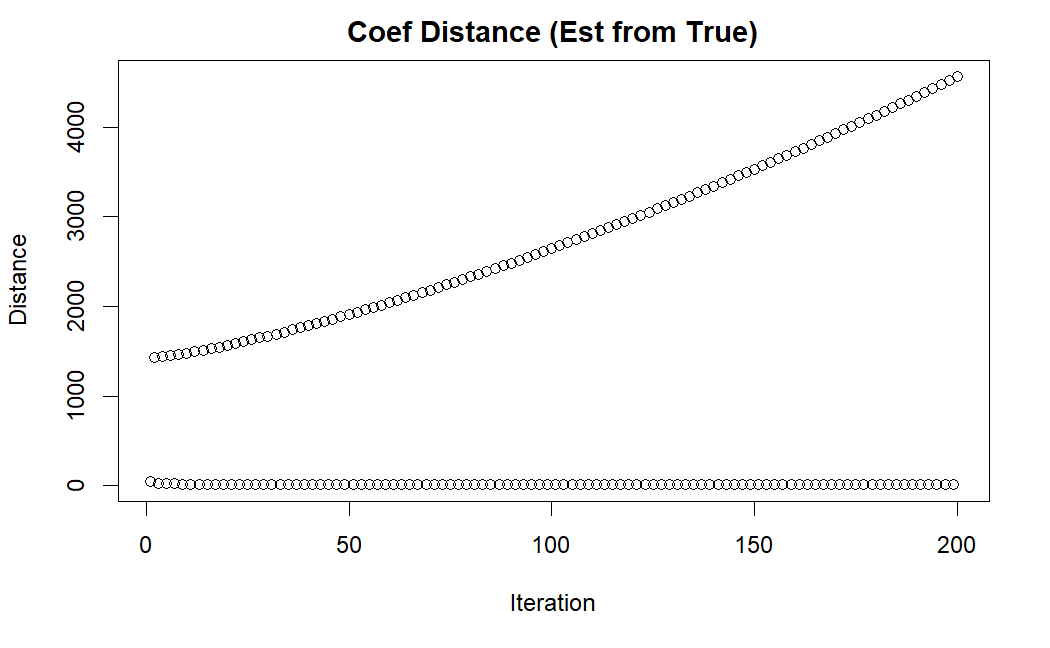
\includegraphics[width=3.5in]{img/beta_gamma_jump.png}
		\end{minipage}%
	}%
	\subfigure[真值+$N(0,1)$初始化]{
		\begin{minipage}[t]{0.5\linewidth}
			\centering
			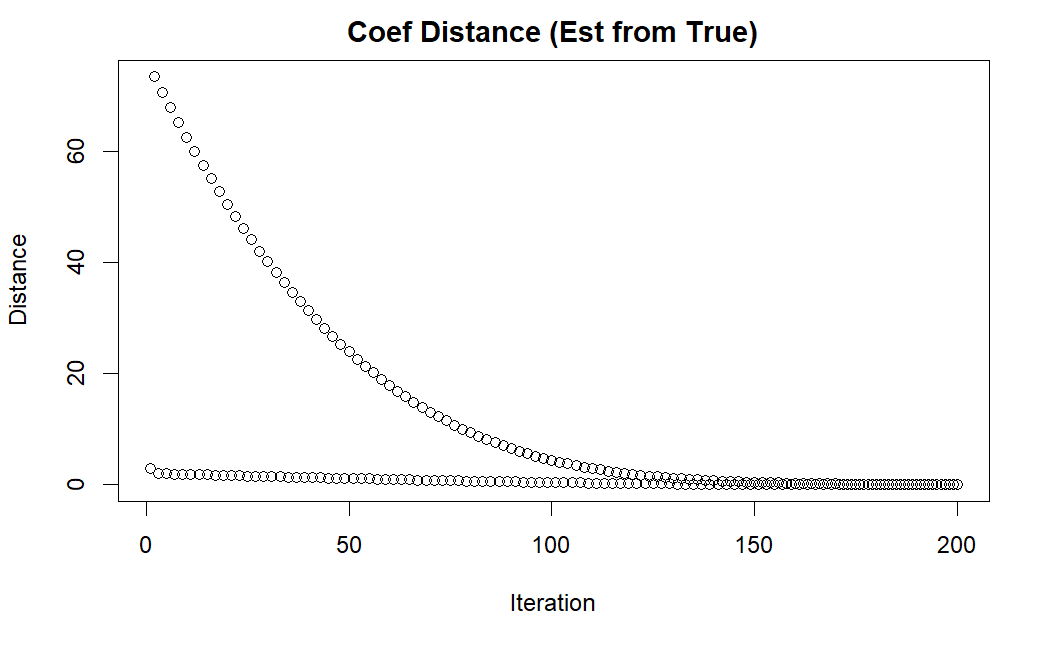
\includegraphics[width=3.5in]{img/beta_gamma_jump2.png}\\
		\end{minipage}%
	}%
	\caption{单类更新 $\beta_k, \gamma_k$ 参数距离真值距离随迭代轮数的变化(使用上一轮结果)}
	\label{fig:beta-gamma-jump}
\end{figure}

\begin{figure}
	\centering
	\subfigure[$N(0,1)$初始化]{
		\begin{minipage}[t]{0.5\linewidth}
			\centering
			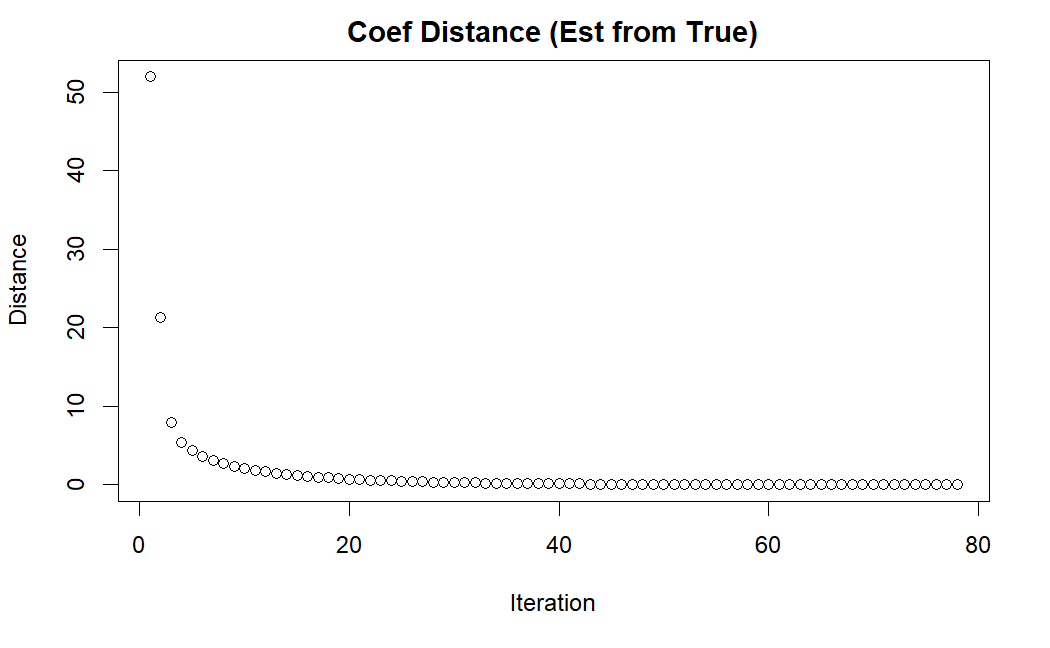
\includegraphics[width=3.5in]{img/beta_gamma_latest.png}
		\end{minipage}%
	}%
	\caption{单类更新 $\beta_k, \gamma_k$ 参数距离真值距离随迭代轮数的变化(使用实时最新结果)}
	\label{fig:beta-gamma-latest}
\end{figure}


由此结论启发,修改参数迭代流程均为使用本轮最新结果进行后续更新,同时更新 $\alpha_k, \beta_k, \gamma_k$ 的结果如图 \ref{fig:one-class-test-old-n200} 所示。



增大 $n=800$ 使得每个类别的 $n_k = 200$ 再使用相同的方法进行一组实验,结果如下,依旧有不收敛的情况,排除 n 小的原因。迭代不收敛时,出现求逆矩阵的最小特征值过小(0.001)的情况,加上 0.1*单位阵项后个别不收敛样例可以收敛,但大多数情况无法改善,排除取逆的矩阵奇异的问题。

参考文章 \cite{wu2020structured},使用新的初始化方法,即 $\beta_k^{(0)}=0, \gamma_k^{(0)}=0$,$\alpha_k^{(0)} = (Z^TZ)^{-1}Z^Ty^{\alpha_k}$。此时不再设计初始化随机策略的问题,对于相同的一组数据只会产生相同的迭代路径和结果。分别使用 $n=200,n=800$ 以及两种初始化策略,得到实验结果如图 \ref{fig:one-class-test-old-n200},\ref{fig:one-class-test-ref-n200},\ref{fig:one-class-test-old-n800},\ref{fig:one-class-test-ref-n800} 所示,样本量 200 或 800 几乎没有影响,但固定初始化(即文献 \cite{wu2020structured} 中的初始化方法)比随机初始化更稳定。更换多组随机种子生成数据进行实验,随机初始化策略中只有真值+$N(0,0.01)$稳定收敛,其他三种随机策略都会出现不收敛或收敛到错误参数的情况,真实计算时无法获取参数真值,故应选择固定初始化策略。

\begin{figure}
	\centering
	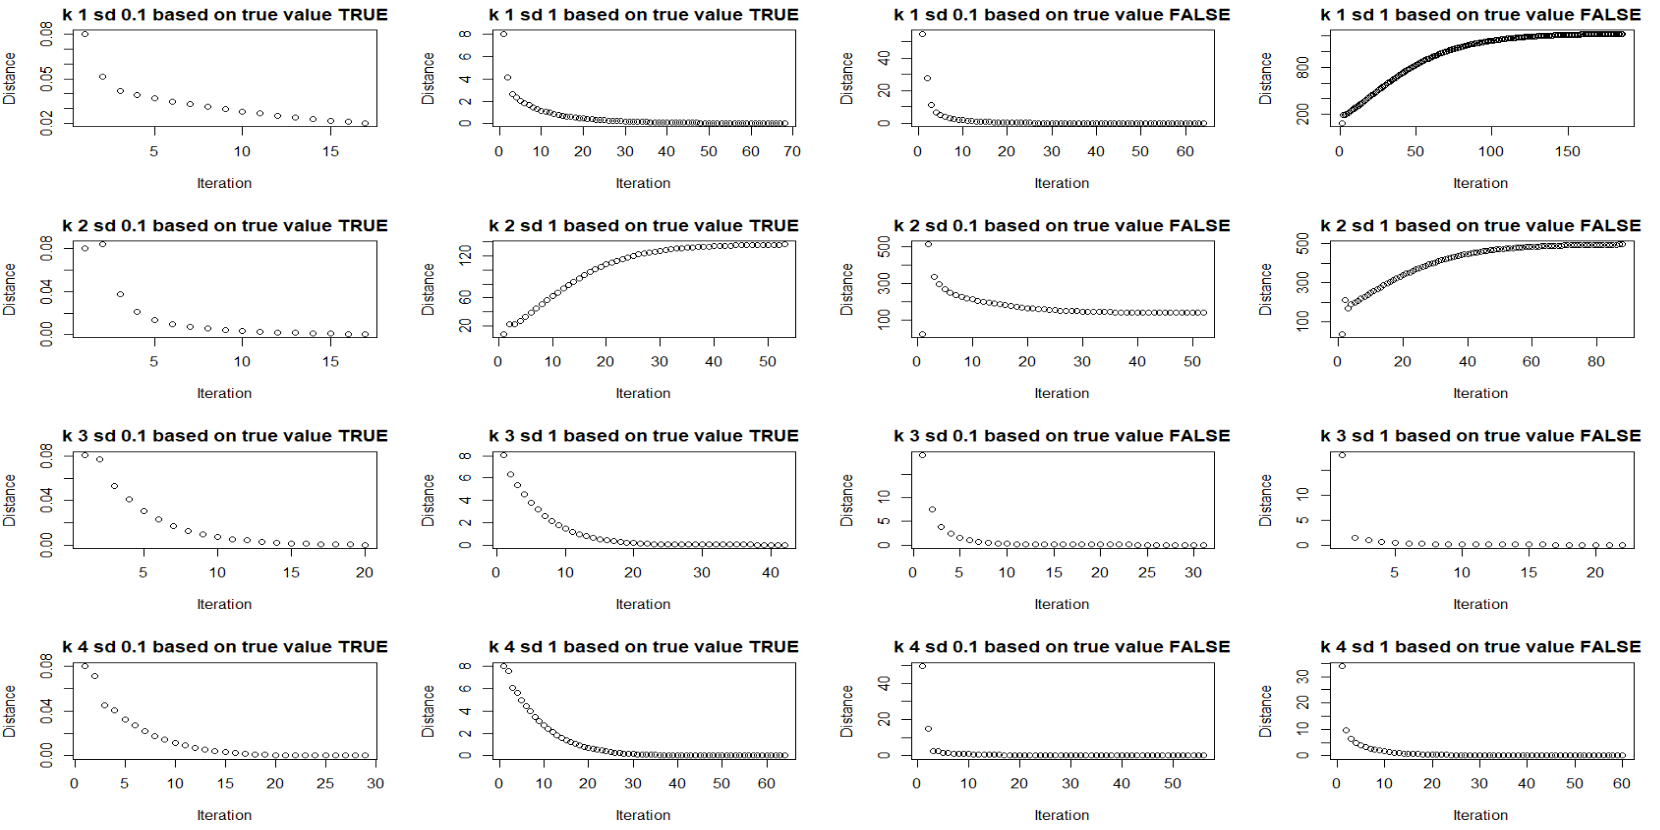
\includegraphics[width=\linewidth]{img/one_class_test_old_n200.png}
	\caption{单类更新参数距离真值距离随迭代轮数的变化(随机初始化),$n=200$}
	\label{fig:one-class-test-old-n200}
\end{figure}

\begin{figure}
	\centering
	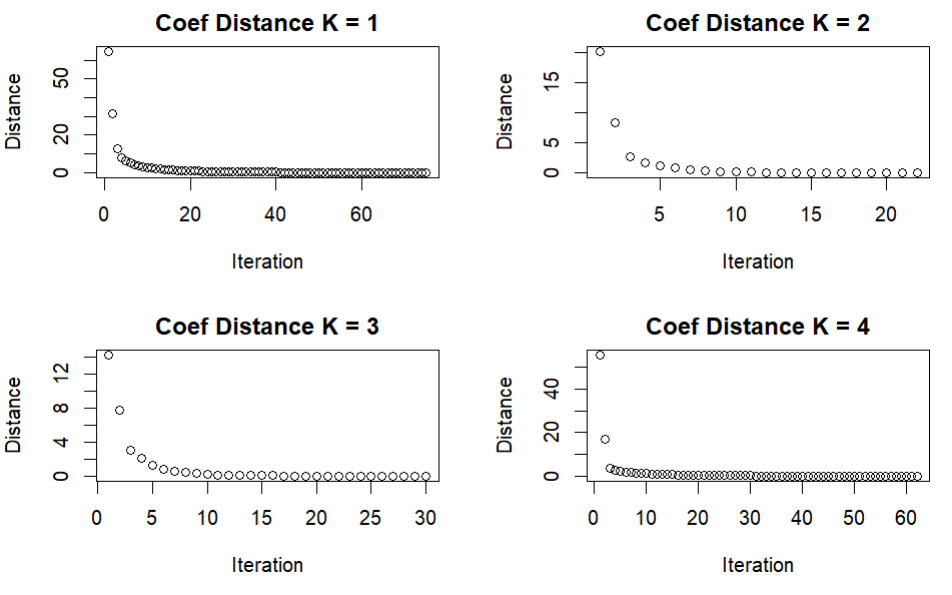
\includegraphics[width=0.8\linewidth]{img/one_class_test_ref_n200.png}
	\caption{单类更新参数距离真值距离随迭代轮数的变化(固定初始化),$n=200$}
	\label{fig:one-class-test-ref-n200}
\end{figure}

\begin{figure}
	\centering
	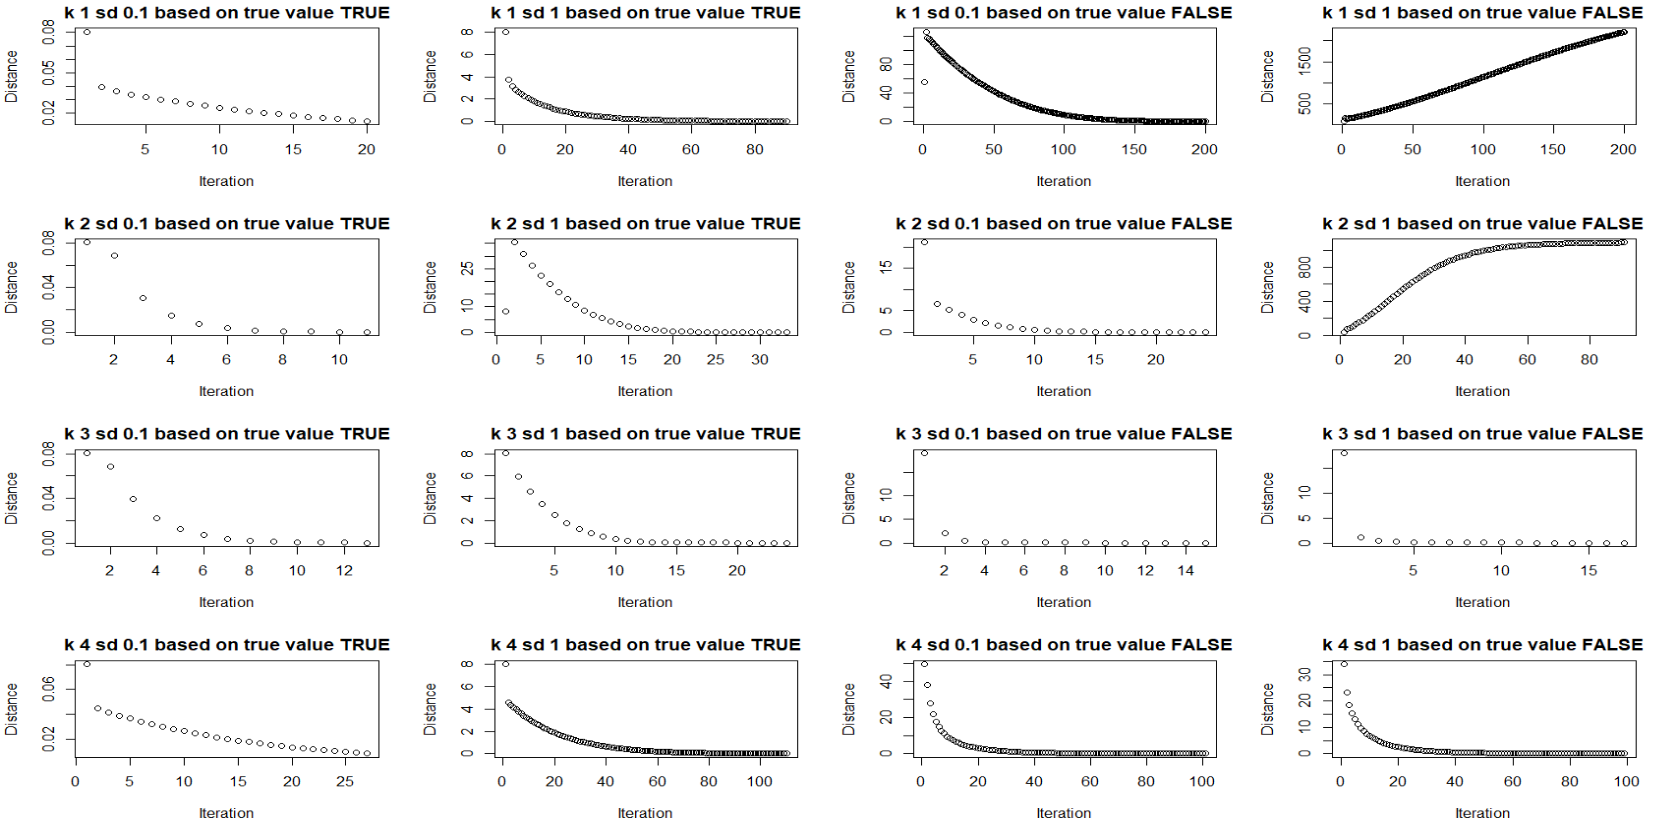
\includegraphics[width=\linewidth]{img/one_class_test_old_n800.png}
	\caption{单类更新参数距离真值距离随迭代轮数的变化(随机初始化),$n=800$}
	\label{fig:one-class-test-old-n800}
\end{figure}

\begin{figure}
	\centering
	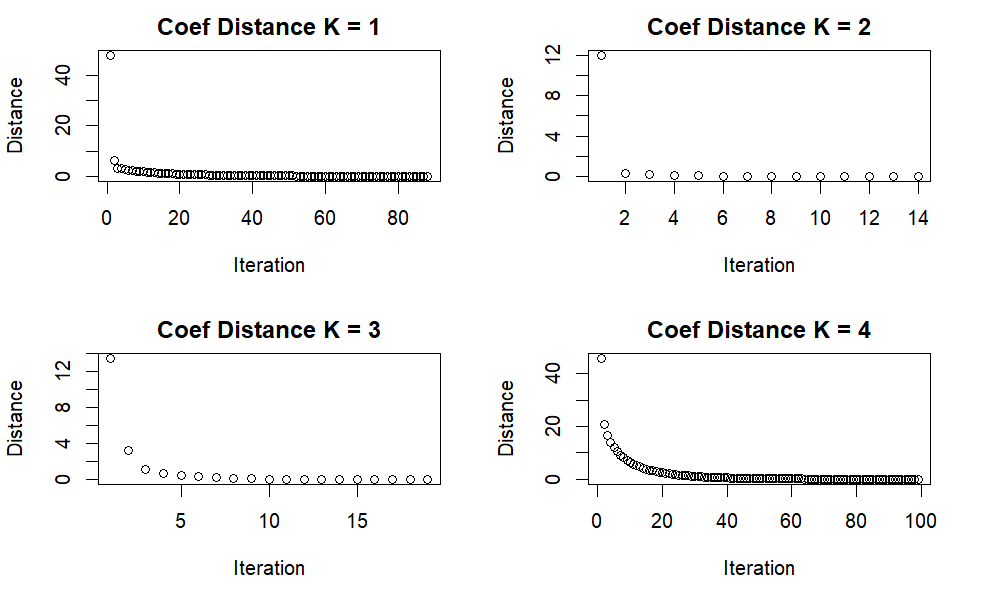
\includegraphics[width=0.8\linewidth]{img/one_class_test_ref_n800.png}
	\caption{单类更新参数距离真值距离随迭代轮数的变化(固定初始化),$n=800$}
	\label{fig:one-class-test-ref-n800}
\end{figure}

固定初始化也不收敛的例子:seed 11,K=4(异常);seed 10,K=1;seed 111,K=1;seed 321,K=2(收敛但到错误值)除 seed 11,K=4 外固定初始化均相对稳定。


以随机种子 11 中的第 4 类为例探究异常原因,经观察发现异常常由 $\gamma_k$ 的过大值导致,图 \ref{fig:theta_res} 反映了对 $(X^{\gamma_k T}W_k X^{\gamma_k} + \theta I)$ 中使用不同的 $\theta$ 对应的迭代结果。

\begin{figure}
	\centering
	\subfigure[$\theta = 0$]{
		\begin{minipage}[t]{0.5\linewidth}
			\centering
			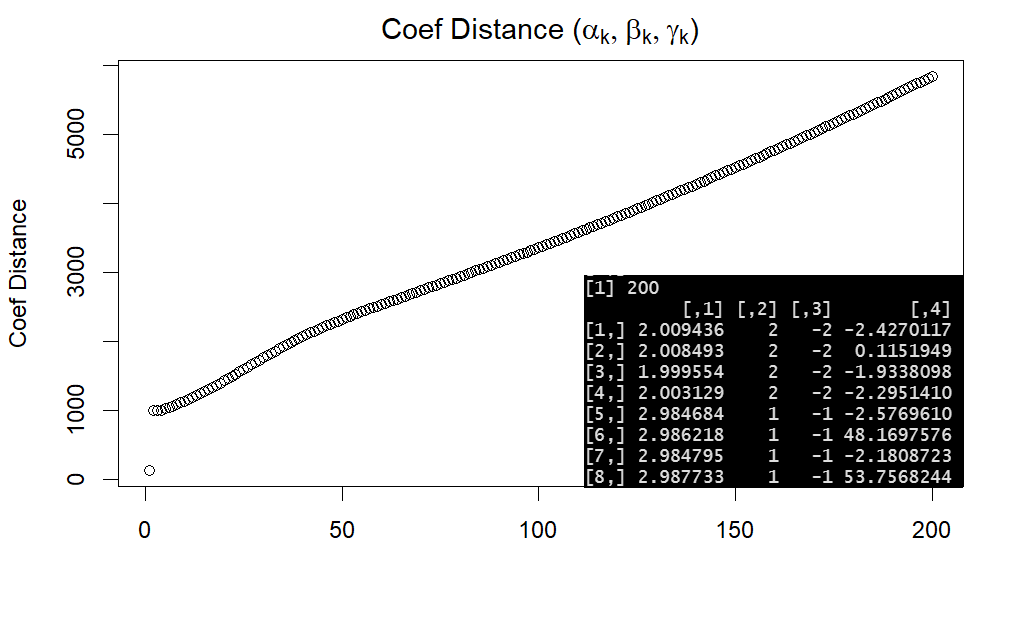
\includegraphics[width=3.5in]{img/theta_all_0.png}
		\end{minipage}%
	}%
	\subfigure[$\theta = 0.1$]{
		\begin{minipage}[t]{0.5\linewidth}
			\centering
			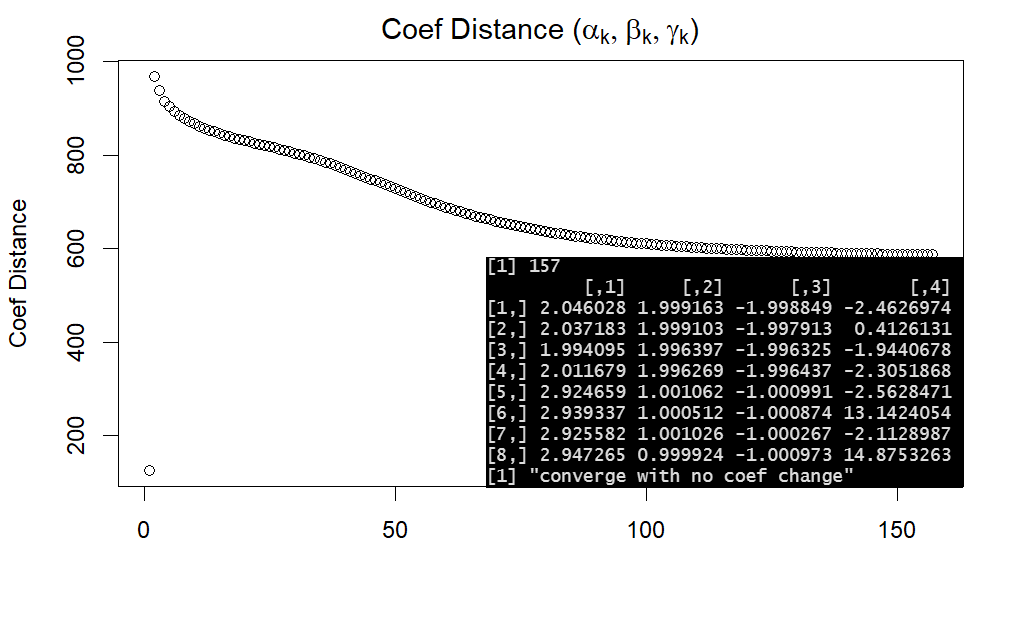
\includegraphics[width=3.5in]{img/theta_all_01.png}
		\end{minipage}%
	}%

\subfigure[$\theta = 1$]{
	\begin{minipage}[t]{0.5\linewidth}
		\centering
		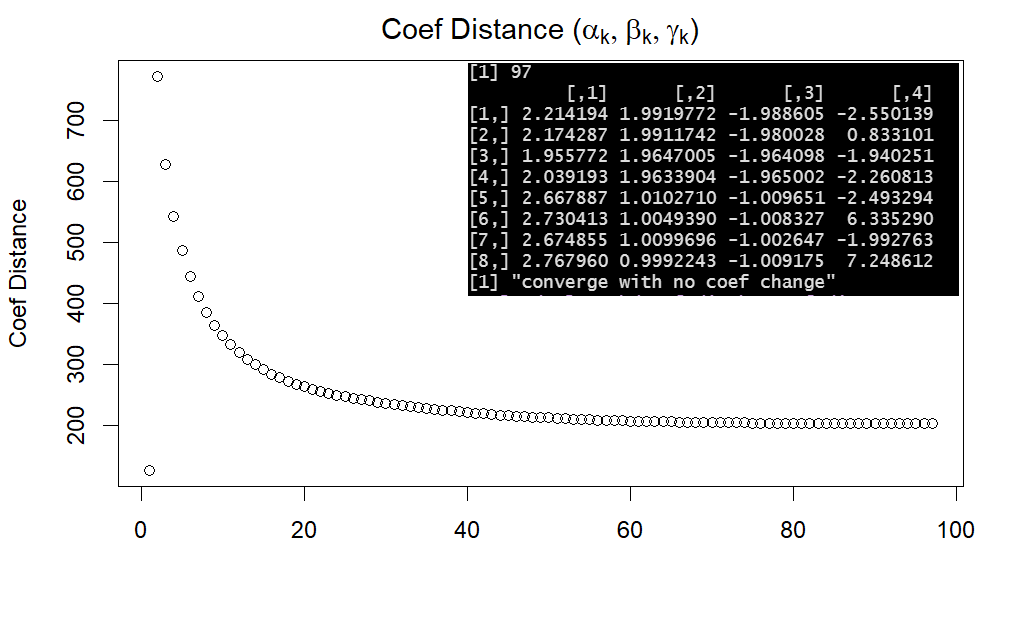
\includegraphics[width=3.5in]{img/theta_all_1.png}
	\end{minipage}%
}%
\subfigure[$\theta_{\gamma} = 1,\theta_{\alpha,\beta} = 0.1$]{
	\begin{minipage}[t]{0.5\linewidth}
		\centering
		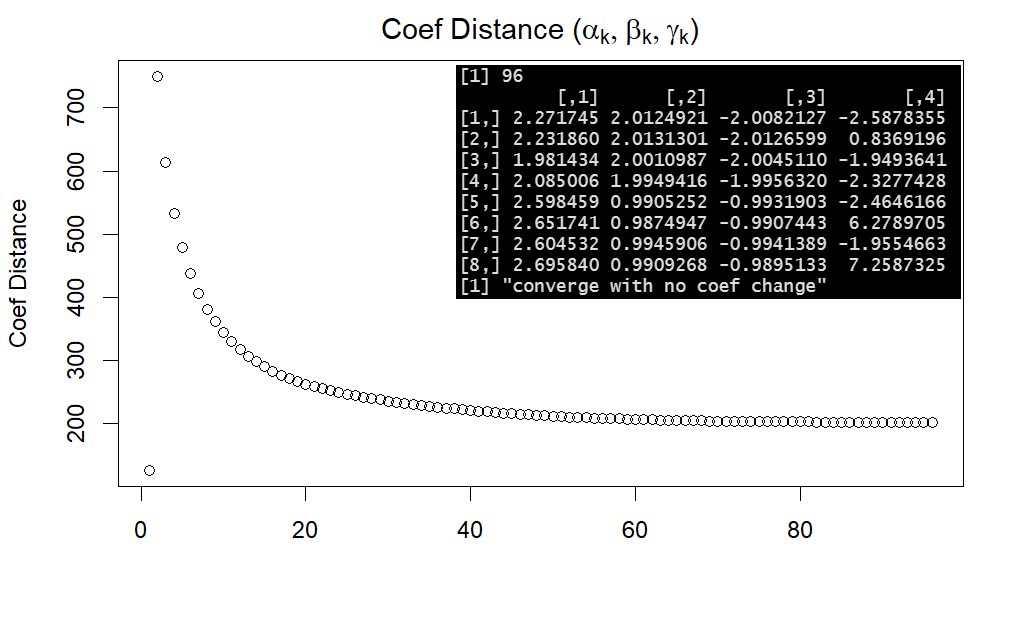
\includegraphics[width=3.5in]{img/theta_gamma.png}
	\end{minipage}%
}%
	\caption{不同 $\theta$ 迭代结果(seed 11)}
	\label{fig:theta_res}
\end{figure}



观察发现,第四类的 $X^T W_k X$ 矩阵特征值特点与其他三类不同,$\beta_k$ 特征值有过大值(2000左右)而 $\gamma_k$ 有相对较小特征值(3左右),而其他类别该矩阵的特征值都是几百的水平,测试其他出现异常的随机种子,均发现类似结论。当前问题重点:加权线性最小二乘系数膨胀问题


其他猜想:自变量的生成机制,但设置均为独立变量也会出现相似问题。


%注意,总使用当前最新的参数可能会改善单个、两个参数收敛,但三个参数不收敛且到真值的距离有明显的往返跳跃性的问题,对于更新单个参数 $\beta_k$ 不收敛到真值没有影响。
\clearpage
\paragraph{四分类给定样本真实归类}

四个分类,真实参数依旧为表 \ref{tb:coef_true} 中的非零项,若给定 $q_{C_i}$ 的真值,即已知每个样本属于哪个分类,检查 $\alpha_k, \beta_k, \gamma_k$ 是否计算正确。

因为 $q_{C_i}$ 的取值在这里只能是 0 或 1,实际计算等价于同时进行四个单类样本计算(已验证)。由表 \ref{tb:one-class-all} 可知相同算法对于不同数据的收敛性是不同的,在固定所属类别的四分类问题中参数的收敛要求各个类别的参数均收敛,即设置参数初始值为真值+$N(0,0.01)$ 时可收敛,其他情况均不收敛。算法的收敛性受初始值影响很大。











\clearpage

\section{Test Summary}

\begin{enumerate}
	\item 初始化参数而非后验概率,EM 算法顺序不可倒置否则无法与原包结果进行对比
	\item $\rho$ 的更新方式,按照类别分和不同类别取平均作每个类别 $1/\sigma$ 效果没有明显差别,为了防止某类异常影响整体效果当前各类别有自己的方差。考虑到及时在最终应用场景中,目标类别也不会太多,这样的设定应该不会增加很大计算复杂度,若有需要再进行调整
\end{enumerate}



\newpage
\bibliographystyle{plain}
\bibliography{ref}

\end{document}